\documentclass{article}
\usepackage[a4paper, total={6in, 8in}]{geometry}
\usepackage[italian]{babel}
\usepackage[T1]{fontenc}
\usepackage{graphicx} 
\usepackage{amsmath}
\usepackage{amssymb}
\usepackage{mathtools}
\usepackage{enumitem}

\begin{document}
\part{Insiemi numerici}
\section{Numeri naturali}
$\mathbb{N} = \{0, 1, 2, ...\}$ \\

\noindent\textbf{NB!} L'insieme $\mathbb{N}$ comprende anche lo 0. \\

\noindent Le operazioni possibili sono l'addizione e la moltiplicazione.

\subsection{Addizione}
\begin{equation*}
    +: \mathbb{N} \times \mathbb{N} \xrightarrow{} \mathbb{N} \qquad \qquad (a,b) \longmapsto a + b
\end{equation*}

\subsubsection{Assiomi}
\noindent\textbf{NB!} Un assioma è una proprietà che vale senza dover essere dimostrata. In altre parole, è presa per vera. \\

\noindent Dati $a, b, c \in \mathbb{N}$, si hanno le seguenti proprietà: 

\begin{itemize}
    \item \textbf{Commutativa}: $a + b = b + a$
    \item \textbf{Associativa}: $(a + b) + c = a + (b + c)$
\end{itemize}

\noindent\textbf{NB!} Si può dimostrare che esiste ed è unico l'elemento neutro $e_0$, cioè quell'elemento che aggiunto ad $a$ non fa cambiare il risultato della somma. Tale elemento è proprio lo 0, infatti:

\begin{equation*}
    a + e_0 = a + 0 = a \qquad \forall a \in \mathbb{N}
\end{equation*}

\subsection{Moltiplicazione}
\begin{equation*}
    \cdot: \mathbb{N} \times \mathbb{N} \xrightarrow{} \mathbb{N} \qquad \qquad (a,b) \longmapsto a \cdot b
\end{equation*}

\subsubsection{Assiomi}
Dati $a, b, c \in \mathbb{N}$, si hanno le seguenti proprietà: 

\begin{itemize}
    \item \textbf{Commutativa}: $a \cdot b = b \cdot a$
    \item \textbf{Associativa}: $(a \cdot b) \cdot c = a \cdot (b \cdot c)$
\end{itemize}

\noindent\textbf{NB!} Si può dimostrare che esiste ed è unico l'elemento neutro $e_1$, cioè quell'elemento che moltiplicato ad $a$ non fa cambiare il risultato. In particolare, si ha che $e_1 = 1$, infatti:

\begin{equation*}
    a \cdot e_1 = a \cdot 1 = a \qquad \forall a \in \mathbb{N}
\end{equation*}

\subsection{Ordinamento totale}
L'insieme $\mathbb{N}$ è totalmente ordinato, ovvero dati due numeri riesco a capire qual è il maggiore e quale il minore. In linguaggio matematico possiamo scrivere: 

\begin{equation*}
    a \leq b \underset{def}{\Longleftrightarrow} \exists \ c \in \mathbb{N} \ | \ a + c = b
\end{equation*}

\noindent\textbf{NB!} Non tutti gli insiemi sono totalmenti ordinati. Ad esempio, i numeri complessi non lo sono.

\subsubsection{Proprietà dell'ordinamento}
\begin{itemize}
    \item \textbf{Riflessiva}: $a \leq a \qquad \forall a \in \mathbb{N}$
    \item \textbf{Antisimmetrica}: è un modo di mostrare che due numeri sono uguali. $$\forall a,b \in \mathbb{N} \quad se \quad \begin{cases}
        a \leq b \\ 
        b \leq a
    \end{cases} \quad allora \quad a = b$$ \noindent Questa è anche la struttura tipica di un \textbf{enunciato}.
    
    \item \textbf{Transitiva}: $\forall a, b, c \in \mathbb{N} \quad se \quad a \leq b \ e \ b \leq c \quad allora \quad a \leq c$.
    \item \textbf{Dicotomia}: $\forall a,b \in \mathbb{N}$, si ha che: $a \leq b \ oppure \ b \leq a$ (essendoci "oppure", significa che o sono entrambe vere o una è vera e l'altra è falsa).
\end{itemize}

\noindent Se ho $\forall a,b,c \in \mathbb{N} \quad a \leq b$, cosa succede se aggiungo $c$? $a +c \leq b + c$. Il segno non cambia grazie alla \textbf{compatibilità dell'ordinamento rispetto alla somma}. \\
Lo stesso vale per la \textbf{compatibilità dell'ordinamento rispetto al prodotto} quando si hanno $\forall a,b,c \in \mathbb{N}, \quad se \quad a \leq b \ e \ c > 0 \implies ac \leq bc$.

\subsection{Struttura di un teorema}
Un teorema possiede sempre: 

\begin{itemize}
    \item un \textbf{enunciato}, avente la seguente struttura: \textit{Se \textbf{ipotesi}, allora \textbf{tesi}};
    \item una \textbf{dimostrazione} dell'enunciato, ovvero un procedimento di deduzione che parte dalla verità delle ipotesi per dimostrare la verità delle tesi.
\end{itemize}

\noindent La dimostrazione può utilizzare l'\textbf{implicazione diretta} del tipo $A \implies B$ oppure l'\textbf{implicazione contronominale} del tipo $\lnot b \implies \lnot a$ (utilizzato nelle dimostrazioni per assurdo/contraddizione). \\
In molti casi, inoltre, si costruisce una contraddizione con un'altra proprietà $c$ (con $c \neq a$):

\begin{equation*}
    \lnot b \implies \begin{cases}
        c \ è \ vero \\
        \lnot c \ è \ vero
    \end{cases}
\end{equation*}

\subsection{Principio di induzione}
\noindent\textbf{NB!} Si chiama "principio", ma è un teorema. \\

\noindent Sia $A \subseteq \mathbb{N}$ e $p \in \mathbb{N}$. Assumiamo che siano valide le seguenti ipotesi: 

\begin{enumerate}
    \item $p \in A$ (questa ipotesi è chiamata \textbf{passo base});
    \item $se \ n \in A \implies n + 1 \in A$ (questa ipotesi è chiamata \textbf{passo induttivo}).
\end{enumerate}

\noindent Allora $\{n \in \mathbb{N} \ | \ n \geq p \} \subseteq A$.

\subsubsection{Esempio 1 di utilizzo del principio di induzione}
Dimostriamo che $\forall n \in \mathbb{N}, \ con \ n \geq 1$, vale: 

\begin{equation}
    \sum_{i = 1}^n i = \frac{n (n + 1)}{2}
\label{eq:1}
\end{equation}

\noindent Lo scopo, quindi, è dimostrare che $A = \{ n \in \mathbb{N} \ |$ (\ref{eq:1}) è vera \}.\\

\noindent Innanzitutto, fissiamo il punto base $p = 1$, essendo che la formula deve essere dimostrata per tutti i numeri naturali $n$, che siano maggiori o uguali a 1. Ma $p = 1 \in A$? Verifichiamolo:

\begin{equation*}
    \sum_{i = 1}^1 i = 1 \qquad \frac{1 \cdot (1 + 1)}{2} = 1
\end{equation*}

\noindent Ciò significa che per $p = 1$, (\ref{eq:1}) è vera, ovvero che il passo base è stato verificato. Ma la formula è vera per tutti $n \in \mathbb{N}$? Non lo so, finché non verifico il passo induttivo, cioè $se \ n \in A \implies n+1 \in A$. Scomponiamo il passo induttivo in ipotesi e tesi ed otteniamo: 

\begin{itemize}
    \item Ipotesi induttiva: $$\sum_{i = 1}^n i = \dfrac{n(n+1)}{2}$$
    \item Tesi induttiva: $$\sum_{i = 1}^{n+1} i = \dfrac{(n+1)(n+2)}{2}$$
\end{itemize}

\noindent Noi ovviamente dobbiamo verificare la tesi. Partiamo quindi da quest'ultima. Attraverso la proprietà associativa della somma possiamo riscriverla come segue:

\begin{equation*}
    \sum_{i = 1}^{n+1} i = \sum_{i = 1}^n i + (n + 1)
\end{equation*}

\noindent Siamo così riusciti a ricondurre il calcolo ad un oggetto noto (l'ipotesi induttiva). Possiamo quindi riscrivere: 

\begin{equation*}
    \sum_{i = 1}^{n+1} i = \frac{n(n+1)}{2} + (n+1)
\end{equation*}

\noindent A questo punto, svolgiamo il denominatore comune e raccogliamo $(n+1)$:

\begin{equation*}
    \sum_{i = 1}^{n+1} i = \frac{(n+1)(n+2)}{2}
\end{equation*}

\noindent Siamo così riusciti a verificare il passo induttivo. Una volta verificato passo base e passo induttivo, possiamo finalmente usare il \textbf{principio di induzione} e quindi dire che $A = \{ n \in \mathbb{N} \ | \ n \geq 1 \}$.

\subsubsection{Esempio 2 di utilizzo del principio di induzione}
Sia $q \in \mathbb{R} - \{ 0, 1 \}$, dimostriamo che: 

\begin{equation}
    \sum_{k = 0}^n q^k = \frac{1-q^{n+1}}{1-q} \quad \forall n \in \mathbb{N}
    \label{eq:2}
\end{equation}

\noindent Poniamo $p = 0$ come passo base (è infatti il valore minimo tra i numeri naturali a cui appartiene $n$) e verifichiamo che esso verifichi la formula: 

\begin{equation*}
    \sum_{k = 0}^n q^k = q^0 = 1 \qquad \frac{1 - q}{1 - q} = 1
\end{equation*}

\noindent Ciò significa che per $p = 0$, (\ref{eq:2}) è vera, ovvero che il passo base è stato verificato. Ma la formula è vera per tutti $n \in \mathbb{N}$? Non lo so, finché non verifico il passo induttivo, cioè $se \ n \in A \implies n+1 \in A$. Scomponiamo il passo induttivo in ipotesi e tesi ed otteniamo: 

\begin{itemize}
    \item Ipotesi induttiva: $$\sum_{k = 0}^n q^k = \frac{1-q^{n+1}}{1-q}$$
    \item Tesi induttiva: $$\sum_{k = 0}^{n + 1} q^k = \frac{1-q^{n+2}}{1-q}$$
\end{itemize}

\noindent Noi ovviamente dobbiamo verificare la tesi. Partiamo quindi da quest'ultima. Attraverso la proprietà associativa della somma possiamo riscriverla come segue:

\begin{equation*}
    \sum_{k = 0}^{n + 1} q^k = \sum_{k = 0}^n q^k + q^{n + 1}
\end{equation*}

\noindent Siamo così riusciti a ricondurre il calcolo ad un oggetto noto (l'ipotesi induttiva). Possiamo quindi riscrivere: 

\begin{equation*}
    \sum_{k = 0}^{n + 1} q^k = \frac{1-q^{n+1}}{1-q} + q^{n + 1}
\end{equation*}

\noindent Svolgiamo ora i calcoli:

\begin{equation*}
    \sum_{k = 0}^{n + 1} q^k = \frac{1-q^{n+1} + q^{n+1} - q\cdot q^{n+1}}{1-q} = \frac{1-q^{n+1} + q^{n+1} - q^{n+2}}{1-q} = \frac{1 - q^{n+2}}{1-q}
\end{equation*}

\noindent Siamo così riusciti a verificare il passo induttivo. Una volta verificato passo base e passo induttivo, possiamo finalmente usare il \textbf{principio di induzione} e quindi dire che $A = \{ n \in \mathbb{N} \ | \ n \geq 0 \}$. Essendo poi che $\mathbb{N}$ contiene già tutti i numeri maggiori o uguali a zero, possiamo direttamente dire che la proprietà è verificata $\forall n \in \mathbb{N}$. \\

\noindent\textbf{NB!} Possiamo estendere la proprietà anche nel caso in cui $q = 0$. Per convenzione, infatti, con i numeri naturali si ha che $0^0 = 1$. Per cui verifichiamo che l'uguaglianza sia ancora mantenuta:

\begin{equation*}
    \sum_{k=0}^n q^k = 0^0 + 0^1 + 0^2 + ... = 1 + 0 + 0 + ... = 1 \qquad \frac{1 - 0^1}{1 - 0} = 1
\end{equation*}

\section{Numeri interi}
$\mathbb{Z} = \mathbb{N} \cup (- \mathbb{N})$ \\

\noindent\textbf{NB!} Per definizione si ha che un "-" insieme equivale a:

\begin{equation*}
    -A \vcentcolon = \{ -a \ | \ a \in A \}
\end{equation*}

\subsection{Assioma di esistenza dell'opposto}
$\forall m \in \mathbb{Z} \ \exists n \in \mathbb{Z} \ | \ m + n = 0$

\subsection{Compatibilità dell'ordinamento}
Se $a,b,c \in \mathbb{Z}$, abbiamo due casi: 

\begin{itemize}
    \item $a \leq b, c > 0 \implies ac \leq bc$
    \item $a \leq b, c < 0 \implies ac \geq bc$
\end{itemize}

\noindent\textbf{Problema!} $a \in \mathbb{Z}, \ \exists b \in \mathbb{Z} \ | \ ab = 1$? Sì, ma ce ne sono solo due: $a \in \{ -1, 1 \}$. In particolare, $b$ è l'inverso del punto $a$. In simboli: $b \vcentcolon = a^{-1}$.

\section{Numeri razionali}
$\mathbb{N} \subsetneq \mathbb{Z} \subsetneq \mathbb{Q}$. In particolare:

\begin{equation*}
    \mathbb{Q} = \{ m \cdot n^{-1} \ | \ m \in \mathbb{Z}, n \in \mathbb{N} - \{ 0 \}, mcd(m,n) = 1 \}
\end{equation*}

\noindent Si nota quindi che $m$ e $n$ sono \textbf{coprimi} perché non hanno divisori comuni (per questo hanno $mcd(m,n) = 1$). \\

\noindent\textbf{NB!} In $\mathbb{Q}$ vale l'\textbf{assioma dell'inverso moltiplicativo} (ovviamente solo per i numeri che me lo permettono. Ad esempio, con 0 non vale), cioè: 

\begin{equation*}
    \forall a \in \mathbb{Q} - \{ 0 \}, \ \exists b \in \mathbb{Q} \ | \ ab = 1 \qquad (dove \ b = a^{-1})
\end{equation*}

\subsection{Dimostrazione di un polinomio senza soluzioni razionali}
\noindent Notiamo ora però che i numeri razionali non ci bastano ancora. Infatti, se prendiamo un polinomio come $p(x) = x^2 - 2$, in cui si ha che $p \in \mathbb{Q}[x]$ (ovvero un polinomio a coefficienti in $\mathbb{Q}$), non si hanno soluzioni razionali per $x^2 - 2 = 0$. Dimostriamo ora per contraddizione questo teorema: \\

\noindent Supponiamo che $\exists \dfrac{m}{n} \in \mathbb{Q} \ | \ \left(\dfrac{m}{n}\right)^2 = 2; \ mcd(m,n) = 1$ (stiamo quindi negando la tesi). Svolgiamo ora dei semplici calcoli:

\begin{equation*}
    \left(\dfrac{m}{n}\right)^2 = 2
\end{equation*}

\begin{equation*}
    \dfrac{m^2}{n^2} = 2
\end{equation*}

\begin{equation*}
    m^2= 2n^2
\end{equation*}

\noindent Essendoci il fattore $2$, $2n^2$ è sicuramente un \textbf{numero pari}, perché può essere diviso per $2$.

\subsubsection{Lemma: un numero elevato al quadrato che è pari è un numero pari}
Immaginiamo di avere un $m$ dispari, che può anche essere scritto come: $m = 2k + 1 \quad con \ k \in \mathbb{Z}$ (ovvero come un numero pari $2k$, trasformato in dispari dall'aggiunta di $1$).\\
Ipotizziamo ora di dover calcolare $m^2$ come nella dimostrazione qui sopra:

\begin{equation*}
    m^2 = (2k + 1)^2 = 4k^2 + 4k + 1 = 4k(k + 1) + 1
\end{equation*}

\noindent Notiamo quindi ancora una volta come, elevando al quadrato un numero dispari $m$, otteniamo nuovamente un numero dispari (perché $4k(k+1)$ è pari, ma è trasformato in dispari dall'aggiunta di $1$).\\

\noindent Ritorniamo ora alla dimostrazione: sapendo che $m^2$ è pari, allora $m$ sarà per forza pari per il lemma qui sopra. Essendo pari, si ha che: $\exists h \in \mathbb{Z} \ | \ m = 2h$ (ovvero stiamo dicendo che $m$ è divisibile per $2$). \\
Riprendiamo ora l'ipotesi di partenza e svolgiamo alcuni calcoli:

\begin{equation*}
    m^2 = 2n^2
\end{equation*}

\begin{equation*}
    (2h)^2 = 2n^2
\end{equation*}

\begin{equation*}
    4h^2 = 2n^2
\end{equation*}

\begin{equation*}
    2h^2 = n^2
\end{equation*}

\noindent Essendo $2h^2$ un numero pari, allora anche $n^2$ è un numero pari e, per lo stesso ragionamento fatto sul lemma, anche $n$ è pari. Arriviamo quindi ad una contraddizione: sia $m$, che $n$ sono numeri pari, ciò significa che $mcd(m,n) \neq 1$ (ovvero non sono numeri coprimi, ma sono in realtà divisibili tra loro). Possiamo così confermare il fatto che non esistono soluzioni razionali a $p(x)$, infatti $\sqrt{2} \notin \mathbb{Z}$. Più in generale, si può dire che $x^2 - p = 0$, dove $p$ è un numero primo, non ha soluzioni razionali ($\sqrt{p} \notin \mathbb{Q})$.\\

\noindent\textbf{NB!} I numeri primi sono i numeri diversi da 1, con fattori solo 1 e se stessi.

\subsection{Fattoriale}
Diamo una definizione induttiva del fattoriale di $n \in \mathbb{N}: n!$: 

\begin{itemize}
    \item $0! = 1$
    \item $(n+1)! \vcentcolon = (n+1)(n!) \qquad \forall n \geq 1$
\end{itemize}

\noindent Per il principio di induzione, $n!$ è ben definito $\forall n \in \mathbb{N}$. \\

\noindent Possiamo anche definirlo come:

\begin{equation*}
    n! = \prod_{i=1}^n i = \vcentcolon 1 \cdot 2 \cdot 3 \cdot 4 \cdot ... \cdot n
\end{equation*}

\subsubsection{Dimostrazione}
Dimostriamo la seguente proposizione: $n! \geq n \quad \forall n \in \mathbb{N}$. Prendiamo innanzitutto un passo base e un passo induttivo:

\begin{itemize}
    \item $p = 0: \quad 0! = 1 \implies 1 \geq 0$. Ciò significa che il passo base è verificato
    \item se $n! \geq n$, allora $(n+1)! \geq (n+1)$
\end{itemize}

\noindent Riscriviamo quindi la tesi, cercando un oggetto noto (l'ipotesi):

\begin{equation*}
    (n+1)! = (n+1)(n!)
\end{equation*}

\noindent Abbiamo già precedentemente dimostrato come $n! \leq n$. Moltiplichiamo ora a destra e a sinistra questa disequazione per $(n+1)$: il verso della disequazione non cambia, essendo che tale numero è sicuramente positivo. Otteniamo quindi:

\begin{equation*}
    (n+1)! = (n+1)(n!) \geq (n+1)n
\end{equation*}

\noindent Avendo quindi mostrato come $(n+1)! \geq (n+1)n$, se riusciamo a dimostrare che $(n+1)n \geq (n+1)$ il gioco è fatto! Essendo che $n \geq 1$, significa che $(n+1) \geq 2$. Capiamo quindi che $(n+1)n \geq (n+1)$ e quindi scritto tutto in una riga:

\begin{equation*}
    (n+1)! \geq (n+1)n \geq (n+1)
\end{equation*}

\subsection{Coefficiente binomiale}
Dati $n, k \in \mathbb{N}$, abbiamo che:

\begin{itemize}
    \item se $k \leq n$: $$\binom{n}{k} \vcentcolon = \dfrac{n!}{k!(n-k)!}$$
    \item se $k > n$: $$\binom{n}{k} \vcentcolon = 0$$
\end{itemize}

\subsubsection{Proprietà del coefficiente binomiale}
\begin{equation*}
    \binom{n}{0} = \frac{n!}{0!(n - 0)!} = \frac{n!}{n!} = 1
\end{equation*}

\begin{equation*}
    \binom{n}{n} = \frac{n!}{n!(n - n)!} = \frac{n!}{n!} = 1
\end{equation*}

\begin{equation*}
    \binom{n}{n-1} = \frac{n!}{(n-1)!(n-(n-1))!} = \frac{n!}{(n-1)!} = \frac{n(n-1)!}{(n-1)!} = n
\end{equation*}

\begin{equation*}
    \binom{n}{k} = \frac{n!}{k!(n-k)!} = \frac{n!}{(n-k)!(n-(n-k))!} = \binom{n}{n-k} \qquad \forall k \leq n
\end{equation*}

\begin{equation*}
    \binom{n}{k} \in \mathbb{N} \quad \forall k,n \in \mathbb{N}
\end{equation*}

\subsubsection{Dimostrazione di una delle proprietà del coefficiente binomiale}
\begin{equation*}
    \binom{n}{k} = \binom{n-1}{k-1} + \binom{n-1}{k}
\end{equation*}

\begin{equation*}
    \binom{n}{k} = \binom{n-1}{k-1} + \binom{n-1}{k} = \frac{(n-1)!}{(k-1)!(n-k)!} + \frac{(n-1)!}{k!(n-1-k)!} \quad con \ 1 \leq k \leq n
\end{equation*}

\begin{equation*}
    \binom{n}{k} = \frac{(n-1)!}{(k-1)!(n-k)(n-k-1)!} + \frac{(n-1)!}{k(k-1)!(n-1-k)!}
\end{equation*}

\begin{equation*}
    \binom{n}{k} = \frac{(n-1)!}{(k-1)!(n-k-1)!} \cdot \left(\frac{1}{n-k} + \frac{1}{k}\right)
\end{equation*}

\begin{equation*}
    \binom{n}{k} = \frac{(n-1)!}{(k-1)!(n-k-1)!} \cdot \left(\frac{n}{k(n-k)}\right)
\end{equation*}

\begin{equation*}
    \binom{n}{k} = \frac{n!}{k!(n-k)!}
\end{equation*}

\section{Numeri reali}
$\mathbb{N} \subsetneq \mathbb{Z} \subsetneq \mathbb{Q} \subsetneq \mathbb{R}$ \\

\noindent\textbf{NB!} Sull'insieme $\mathbb{R}$ valgono tutti gli assiomi definiti precedentemente!

\subsection{Assioma di separazione}
Prendiamo due insiemi $A$ e $B$ con $A \neq \varnothing \neq B$ tali che $a \leq b \quad \forall a \in A, \forall b \in B$ (dato che tutti gli elementi di $A$ sono più piccoli di quelli di $B$, i due insiemi si dicono \textbf{separati}), allora: 

\begin{equation*}
    \exists x \in \mathbb{R} \ | \ a \leq x \leq b \quad \forall a \in A, \forall b \in B
\end{equation*}

\noindent dove $x$ è detto \textbf{separatore} di $A$ e $B$.

\subsection{Proprietà di Archimede con relativa dimostrazione}
\begin{equation*}
    \forall x \in \mathbb{R}, \exists n \in \mathbb{N} \ | \ n > x
\end{equation*}

\noindent Dimostriamo per contraddizione questa proprietà. Innanzitutto verifichiamo il caso in cui $x \leq 0$. Dal momento che $\mathbb{N}$ contiene numeri maggiori o uguali a 0, la proprietà è già verificata. \\
Studiamo ora il caso in cui $x > 0$: definiamo l'insieme $A$ come segue: $A \vcentcolon = \{ n \in \mathbb{N} \ | \ n \leq x \} \subseteq \mathbb{N}$. La nostra tesi è che $A \neq \mathbb{N}$, cioè che $\exists m \notin A$ (perché $m > x$). Supponiamo allora che $A = \mathbb{N} \neq \varnothing$. Sia ora $B \vcentcolon = \{ y \in \mathbb{R} \ | \ y \geq n, \forall n \in \mathbb{N} \}$. Se $A = \mathbb{N}$, allora tutti i numeri naturali sono più piccoli di $x$. Per questo motivo possiamo dire che $x$ "fa il gioco" di $y$ (ovvero è un numero reale, maggiore di tutti i numeri naturali). Quindi $x \in B$, per cui ne deriva che $B \neq \varnothing$. \\
Dato che $\forall y \in B$ si ha che $y \geq n \quad \forall n \in A \ (= \mathbb{N})$, allora significa che $A$ e $B$ sono insiemi separati. Per questo motivo, possiamo sfruttare l'assioma di separazione: $\exists \lambda \in \mathbb{R} \ | \ n \leq \lambda \leq y \quad \forall n \in A \ (= \mathbb{N}), \forall y \in B$. Dato che $n+1 \in \mathbb{N}$, è vero che $n+1 \leq \lambda \leq y$. \\
Concentriamoci ora sulla prima parte della disequazione $n+1 \leq \lambda$ e riscriviamola come $n \leq \lambda - 1 \quad \forall n \in A \ (= \mathbb{N})$. Dato che $\lambda$ è un numero reale maggiore o uguale di ogni numero naturale, anche $\lambda - 1$ lo è. Per cui possiamo dire che $\lambda - 1 \in B$. Infine, per definizione $\lambda$ è elemento separatore di $A$ e $B$, quindi: $(n \leq) \ \lambda \leq y \quad \forall y \in B, \forall n \in A$. Quindi, possiamo sostituire il generico elemento $y$ di $B$, con $\lambda - 1$ e otteniamo $\lambda \leq \lambda - 1 \implies 1 \leq 0$, che è una contraddizione.

\subsection{Proprietà della parte intera}
$\forall x \in \mathbb{R}, \ \exists ! \ n \in \mathbb{Z} \ | \ n \leq x < n + 1$ \\

\noindent\textbf{NB!} $n$ è detto \textbf{parte intera} di $x$ e si indica con $n = \lfloor x \rfloor$.

\subsubsection{Grafici della parte intera}
\begin{figure}[!h]
    \centering
    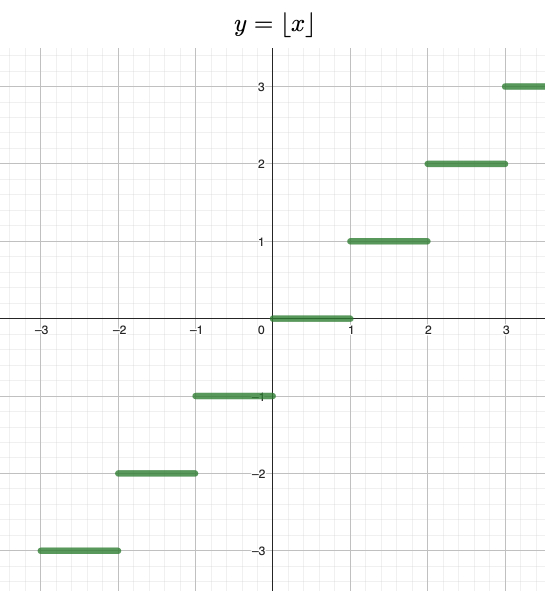
\includegraphics[width=7cm]{./images/floor_graph.jpg}\hfill
    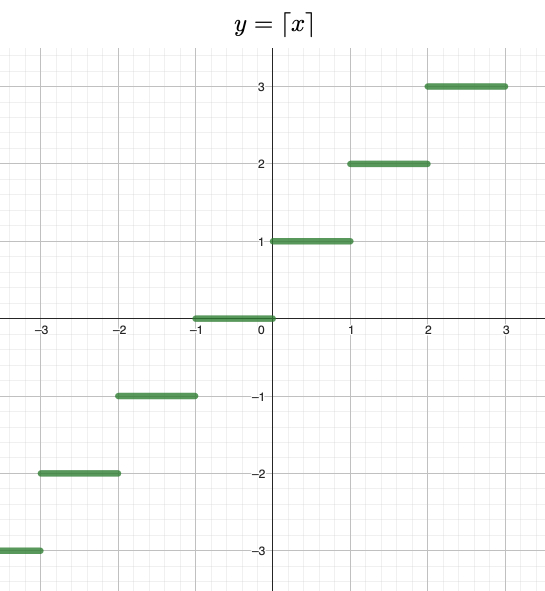
\includegraphics[width=7cm]{./images/ceil_graph.jpg}
\end{figure}

\noindent \textbf{NB!} Non è vero che $\lceil x \rceil = \lfloor x \rfloor + 1 \quad \forall x \in \mathbb{R}$, ma è vero solo per $x \in \mathbb{R} - \mathbb{Z}$.

\subsection{Teorema della densità dei razionali nei reali e relativa dimostrazione}
\begin{center}
    $\forall x \in \mathbb{R}, \forall \varepsilon > 0, \exists z \in \mathbb{Q} \ | \ z \leq x < z + \varepsilon \quad dove \ \varepsilon \in \mathbb{R}$
    \begin{figure}[!h]
    \centering
    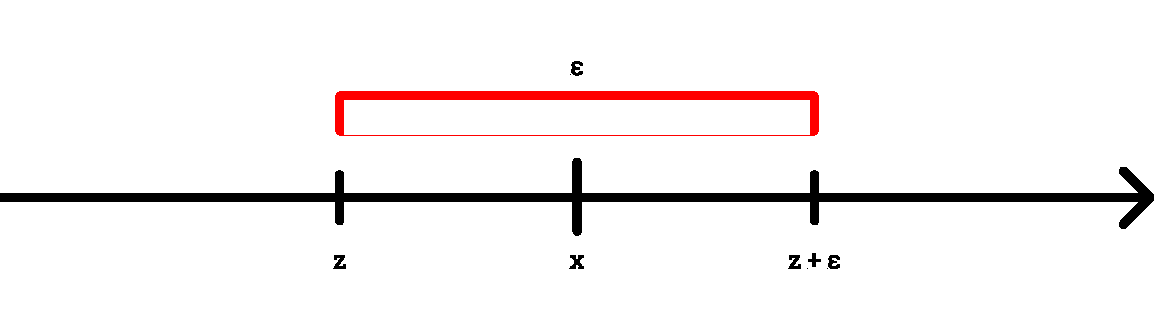
\includegraphics[width=15cm]{./images/densityQinR.pdf}
\end{figure}
\end{center}

\noindent Dimostriamo ora questo teorema. Sia $x \in \mathbb{R}, \varepsilon > 0$. Allora $\dfrac{1}{\varepsilon} > 0$. Utilizziamo ora la proprietà di Archimede:

\begin{equation*}
    \exists q \in \mathbb{N} \ | \ q > \frac{1}{\varepsilon} > 0
\end{equation*}

\noindent Consideriamo ora $qx \in \mathbb{R}$ e usiamo la proprietà della parte intera: 

\begin{equation*}
    \exists p \in \mathbb{N} \ | \ p \leq qx < p + 1
\end{equation*}

\noindent Dividiamo ora per $q$ (essendo $q > 0$, il verso della disequazione non cambia): 

\begin{equation*}
    \frac{p}{q} \leq x < \frac{p}{q} + \frac{1}{q} \qquad dove \ \frac{p}{q} \in \mathbb{Q}
\end{equation*}

\noindent Ma essendo che $q > \dfrac{1}{\varepsilon}$ per la proprietà di Archimede, possiamo anche dire che $q\varepsilon > 1$ e che $\varepsilon > \dfrac{1}{q}$. Ne segue quindi che: 

\begin{equation*}
    \frac{p}{q} \leq x < \frac{p}{q} + \varepsilon \qquad dove \ \frac{p}{q} = z
\end{equation*}

\subsection{Teorema}
Se $a, b \in \mathbb{R}$ con $a < b$, allora: 

\begin{itemize}
    \item $\exists r \in \mathbb{Q} \ | \ a < r < b$ (ovvero tra due numeri reali, c'è sempre un razionale, purché $a \neq b$);
    \item $\exists \alpha \in \mathbb{R} - \mathbb{Q} \ | \ a < \alpha < b$ (ovvero tra due numeri reali, c'è sempre un irrazionale, purché $a \neq b$).
\end{itemize}

\subsection{Intervalli}
Esistono tre tipi di intervalli: 

\begin{itemize}
    \item \textbf{intervalli aperti}: $(a,b) = \{ x \in \mathbb{R} \ | \ a < x < b \}$;
    \item \textbf{intervalli semichiusi}: $(a,b] = \{ x \in \mathbb{R} \ | \ a < x \leq b \}$ oppure $[a,b) = \{ x \in \mathbb{R} \ | \ a \leq x < b \}$;
    \item \textbf{intervalli chiusi}: $[a,b] = \{ x \in \mathbb{R} \ | \ a \leq x \leq b \}$.
\end{itemize}

\noindent Dato $A \subseteq \mathbb R$ con $A \neq \varnothing$, $A$ si dice intervallo se e solo se $\forall x_1, x_2 \in A, \ x_1 < x_2$ si ha che $\{ x \in \mathbb{R} \ | \ x_1 < x < x_2 \} \subset A$. \\
Ad esempio, $A = (0,1) \cup \{2\}$ non è un intervallo perché se prendo $x_1 = \dfrac{1}{2}$ e $x_2 = 2$, noto come $x = \dfrac{3}{2} \notin A$. 

\subsection{Maggioranti-minoranti, insiemi superiormente-inferiormente limitati}
Dato $A \subseteq B$ con $A \neq \varnothing$, diremo che:

\begin{enumerate}
    \item $x \in \mathbb{R}$ è \textbf{maggiorante} di $A$ se e solo se $a \leq x \quad \forall a \in A$;
    \item $x \in \mathbb{R}$ è \textbf{minorante} di $A$ se e solo se $a \geq x \quad \forall a \in A$.
\end{enumerate}

\noindent Diremo quindi che $A$ è inferiormente (superiormente) limitato se e solo se esiste un minorante (maggiorante) di A. \\
Ad esempio, se $A = (0,1) \cup \{2\}$, esso è un insieme inferiormente limitato da 0 (minorante) e superiormente limitato da 2 (maggiorante). Si dice perciò che è un insieme \textbf{limitato}.

\subsubsection{Proprietà degli insiemi inferiormente/superiormente limitati}
Sia $A \subseteq \mathbb{R}$ con $A \neq \varnothing$. Se $A$ è inferiormente limitato, allora $B \subseteq A$ è anch'esso inferiormente limitato. \\

\noindent Dimostriamo questa proprietà. Dato che $A$ è inferiormente limitato, significa che esso possiede un minorante, in simboli $\exists x \in \mathbb{R} \ | \ x \leq a \quad \forall a \in A$. Ora, se un punto $b \in B$, allora $b \in A$ perché $B \subseteq A$. Proprio per questo motivo, $x \leq b \quad \forall b \in B \subseteq A$. Allora $x$ è un minorante di $B$ e quindi $B$ è inferiormente limitato. \\

\noindent Dimostriamo ora il caso di un insieme superiormente limitato. Dato quindi che $A$ è superiormente limitato, esso possiede un maggiorante, in simboli $\exists x \in \mathbb{R} \ | \ x \geq a \quad \forall a \in A$. Ora, se un punto $b \in B$, allora $b \in A$ perché $B \subseteq A$. Proprio per questo motivo, $x \geq b \quad \forall b \in B \subseteq A$. Allora $x$ è un maggiorante di $B$ e quindi $B$ è superiormente limitato.

\subsubsection{Insieme $\mathbb{N}$: inferiormente-superiormente limitato?}
Dato che i numeri naturali soddisfano la seguente condizione $n \geq 0 \quad \forall n \in \mathbb{N}$, significa che 0 è un minorante di $\mathbb{N}$ e che perciò $\mathbb{N}$ è inferiormente limitato.\\
Ma $\mathbb{N}$ è superiormente limitato? Se fosse vero, significherebbe che $\exists x \in \mathbb{R} \ | \ n \leq x \quad \forall n \in \mathbb{N}$, ma ciò va in contraddizione con la proprietà di Archimede. Perciò $\mathbb{N}$ non è superiormente limitato.

\subsubsection{Insieme $\mathbb{Z}$: inferiormente-superiormente limitato?}
Dato che $\mathbb{N}$ non è superiormente limitato e che $\mathbb{N} \subseteq \mathbb{Z}$, ne segue che neanche $\mathbb{Z}$ è superiormente limitato.\\

\noindent Ma $\mathbb{Z}$ è inferiormente limitato? Supponiamo che lo sia, ovvero che $\exists b \in \mathbb{R} \ | \ b \leq z, \forall z \in \mathbb{Z}$. Essendo che $\mathbb{Z}$ è composto anche da numeri negativi, sappiamo che $b$ deve essere sicuramente negativo ($b < 0$). Ne segue che $-b > 0$. Quindi riprendendo il ragionamento:

\begin{equation*}
    b \leq z \implies -b \geq -z \quad \forall z \in \mathbb{Z} \iff -b \geq w \quad \forall w \in \mathbb{Z}
\end{equation*}

\noindent Arriviamo così ad una contraddizione perché stiamo dicendo che $-b$, un numero positivo, è minorante di $\mathbb{Z}$, quando sappiamo benissimo che esso contiene anche numeri negativi. Per questo motivo, possiamo concludere che $\mathbb{Z}$ non è inferiormente limitato.

\subsubsection{Insieme $\mathbb{Q}$: inferiormente-superiormente limitato?}
Dato che né $\mathbb{N}$, né $\mathbb{Z}$ sono superiormente limitati, allora nemmeno $\mathbb{Q}$ è superiormente limitato. Inoltre, dato che $\mathbb{Z}$ non è inferiormente limitato, allora nemmeno $\mathbb{Q}$ è inferiormente limitato.

\subsubsection{Insieme $\mathbb{R}$: inferiormente-superiormente limitato?}
Dato che $\mathbb{N}$, $\mathbb{Z}$ e $\mathbb{Q}$ non sono superiormente limitati, allora nemmeno $\mathbb{R}$ è superiormente limitato. Inoltre, dato che né $\mathbb{Z}$, né $\mathbb{Q}$ sono inferiormente limitati, allora nemmeno $\mathbb{R}$ è inferiormente limitato.

\subsection{Massimi e minimi}
\textbf{Def:} Sia $A \subseteq R, A \neq \varnothing$, allora diremo che $A$ ammette massimo (minimo) se e solo se

\begin{equation*}
    \exists x_0 \in A \ | \ x_0 \geq a \ (x_0 \leq a) \quad \forall a \in A
\end{equation*}

\noindent In altre parole, se $x_0$ è maggiorante (minorante) di $A$ ed esso appartiene ad $A$, allora $x_0$ sarà un massimo (minimo).\\

\noindent\textbf{ES.} Prendiamo, ad esempio, $A = (0, 1]$. Sicuramente, ogni $x \geq 1$ sarà un maggiorante di $A$, ovvero:

\begin{equation*}
    M_A \vcentcolon = \{ x \in \mathbb{R} \ | \ x \ è \ maggiorante \ di \ A \} = \{ x \in \mathbb{R} \ | \ x \geq 1 \}
\end{equation*}

\noindent Ciò significa che:

\begin{itemize}
    \item Se $x \geq 1 \implies x \in M_A$
    \item Se $x \in M_A \implies x \geq 1$
\end{itemize}

\noindent Dato che nell'insieme dei maggioranti si ha che $x \geq 1$ e che $1 \in A \implies max(A) = 1$ (perché appunto $1 \in M_A$ e $1 \in A$).\\

\noindent Per quanto riguarda i minoranti, si ha che:

\begin{equation*}
    m_a \vcentcolon = \{ x \in \mathbb{R} \ | \ x \ è \ minorante \ di \ A \} = \{ x \in \mathbb{R} \ | \ x \leq 0 \}
\end{equation*}

\noindent Dato che $A: 0 < x \leq 1$ e $m_a: x \leq 0 \implies \nexists \ min(A)$.\\

\noindent\textbf{NB!} Non è detto che un insieme abbia sempre un massimo o un minimo.

\subsection{Legami tra massimi, minimi ed insiemi limitati}
\textbf{Teorema:} Sia $A \subseteq \mathbb{R}, A \neq \varnothing$. Allora:

\begin{enumerate}[label=\alph{enumi})]
    \item Se $A$ è \textbf{superiormente limitato} $\implies$ $M_A$ ammette \textbf{minimo} ($1$ nell'esempio di prima);
    \item Se $A$ è \textbf{inferiormente limitato} $\implies$ $m_A$ ammette \textbf{massimo} ($0$ nell'esempio di prima).
\end{enumerate}

\noindent\textbf{Def:} $A \subseteq \mathbb{R}, A \neq \varnothing$:

\begin{enumerate}
    \item Se $A$ è \textbf{inferiormente limitato} chiamo \textbf{estremo inferiore} di $A$ ($inf(A)$) il $max(m_A)$;
    \item Se $A$ è \textbf{superiormente limitato} chiamo \textbf{estremo superiore} di $A$ ($sup(A)$) il $min(M_A)$;
    \item Se $A$ \textbf{non} è \textbf{superiormente limitato}, scriviamo che $sup(A) = + \infty$;
    \item Se $A$ \textbf{non} è \textbf{inferiormente limitato}, scriviamo che $inf(A) = - \infty$.
\end{enumerate}

\noindent\textbf{NB!} $\pm \infty$ non sono numeri reali, perciò non è possibile eseguire operazioni con essi.

\subsubsection{Dimostrazione del teorema qui sopra enunciato}
Dimostriamo innanzitutto il primo punto. Per ipotesi, $A$ è superiormente limitato, cioè $\forall a \in A, \forall y \in M_A (\neq \varnothing)$, si ha che $a \leq y$. Dato che $A \neq \varnothing$ e che $M_A \neq \varnothing$, essi sono separati. Per questo motivo, possiamo usare l'assioma di separazione e dire che:

\begin{equation*}
    \exists b \in \mathbb{R} \ | \ a \leq b \leq y \qquad \forall a \in A, \forall y \in M_A    
\end{equation*}

\noindent Essendo che $a \leq b \quad \forall a \in A \implies b \in M_A$ (cioè $b$ è un maggiorante) e che $b \leq y \quad \forall y \in M_A \implies b = min(M_A) \implies b$ è l'estremo superiore. \\

\noindent Dimostriamo ora il secondo punto. Per ipotesi, $A$ è inferiormente limitato, cioè $\forall a \in A, \forall y \in m_A (\neq \varnothing)$, si ha che $a \geq y$. Dato che $A \neq \varnothing$ e che $m_A \neq \varnothing$, essi sono separati. Per questo motivo, possiamo usare l'assioma di separazione e dire che: 

\begin{equation*}
    \exists b \in \mathbb{R} \ | \ y \leq b \leq a \qquad \forall a \in A, \forall y \in m_A
\end{equation*}

\noindent Essendo che $b \leq a \quad \forall a \in A \implies b \in m_A$ (cioè $b$ è un minorante) e che $b \geq y \quad \forall y \in m_A \implies b = max(m_A) \implies b$ è l'estremo inferiore. \\

\noindent\textbf{Osservazione:} Con $A \neq \varnothing$ si ha che:

\begin{enumerate}[label=\alph{enumi})]
    \item se $sup(A) \in A \implies sup(A) = max(A)$;
    \item se $inf(A) \in A \implies inf(A) = min(A)$.
\end{enumerate}

\noindent\textbf{NB!} Come detto precedentemente, è possibile che un insieme non abbia massimi o minimi, ma ha \textbf{sempre} estremi superiori e inferiori. \\

\noindent\textbf{Teorema - Caratterizzazione di estremi inferiori e superiori reali:} Sia $A \neq \varnothing, A \subseteq \mathbb{R}$. Allora:

\begin{enumerate}[label=\alph{enumi})]
    \item se $A$ è superiormente limitato, allora: 
    \begin{equation*}
        x = sup(A) \iff \begin{cases}
            x \geq a \qquad \forall a \in A \ (x \in M_A) \\
            \forall \varepsilon > 0, \exists \Bar{a} \in A \ | \ \Bar{a} > x - \varepsilon
        \end{cases}
    \end{equation*}
    \item se $A$ è inferiormente limitato, allora:
    \begin{equation*}
        x = inf(A) \iff \begin{cases}
            x \leq a \qquad \forall a \in A \ (x \in m_A) \\
            \forall \varepsilon > 0, \exists \Bar{a} \in A \ | \ \Bar{a} < x + \varepsilon
        \end{cases}
    \end{equation*}
\end{enumerate}

\noindent Ciò significa che ci saranno elementi di $A$ arbitrariamente vicini all'estremo superiore/inferiore. Graficamente:

\begin{center}
    \begin{figure}[!h]
        \centering
        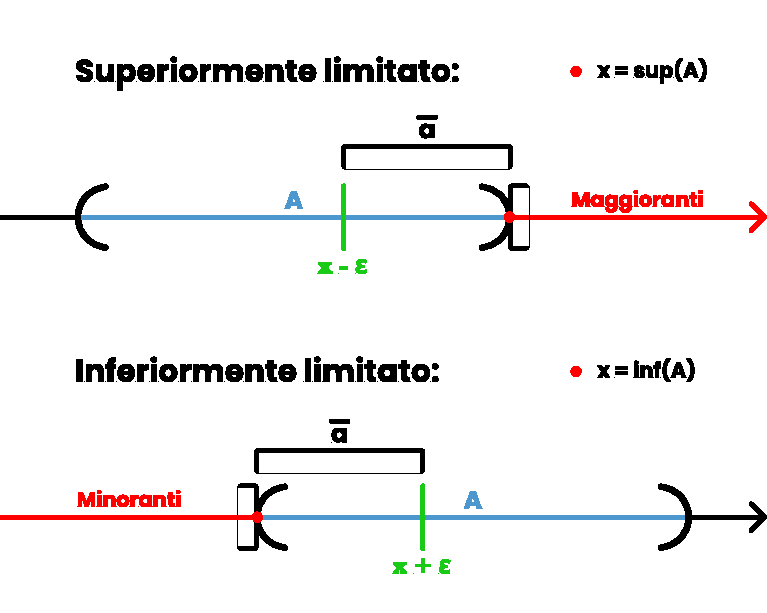
\includegraphics[width=8cm]{./images/infSupTheorem.pdf}
    \end{figure}
\end{center}

\noindent Dimostriamo ora l'implicazione ($\Rightarrow$) del punto a). Per ipotesi, sappiamo che $x = sup(A) \in \mathbb{R}$, allora $x \in M_A$ quindi $x \geq a \quad \forall a \in A$. In particolare, $x = min(M_A)$. \\
Sia $\varepsilon > 0$, allora $x - \varepsilon < x \implies x - \varepsilon \notin M_A$ (perché è più piccolo del minimo, cioè $x$). Dato che $\alpha \in M_A \underset{def}{\Longleftrightarrow} \alpha \geq a \quad \forall a \in A$, ma $\alpha \notin M_A$ (ovvero $\alpha \geq a \quad \forall a \in A$ è falsa). Possiamo dire che $\exists \Bar{a} \in A \ | \ \alpha < \Bar{a}$. Quindi $x - \varepsilon \notin M_A$ e posso scrivere che $\exists \Bar{a} \in A \ | \ x - \varepsilon < \Bar{a}$.\\
Dimostriamo ora la controimplicazione ($\Leftarrow$). Le ipotesi sono le seguenti:

\begin{enumerate}[label=\roman*)]
    \item $A$ è superiormente limitato;
    \item $x \geq a \quad \forall a \in A$;
    \item $\forall \varepsilon > 0, \exists \Bar{a} \in A \ | \ \Bar{a} > x - \varepsilon$
\end{enumerate}

\noindent La tesi da dimostrare è, invece, $x = sup(A)$. Per la seconda ipotesi (ii), capiamo che $x \in M_A$. Mentre dalla terza (iii) abbiamo che $x - \varepsilon \notin M_A \quad \forall \varepsilon > 0$ (cioè $x - \varepsilon$ non è un maggiorante). Segue quindi che:

\begin{equation}
    min(M_A) > x - \varepsilon \quad \forall \varepsilon > 0
    \label{eq:3}
\end{equation}

\noindent Sia ora $y = min(M_A)$, se fosse $y < x \implies \exists \Bar{\varepsilon} \ | \ y \leq x - \Bar{\varepsilon}$ che contraddice la (\ref{eq:3}). Pertanto, $y = min(M_A) \geq x$. Allora $x = min(M_A)$, ossia $x = sup(A)$.\\

\noindent Alla stessa maniera, dimostriamo ora il punto b). Partiamo dall'implicazione ($\Rightarrow$). Per ipotesi, sappiamo che $x = inf(A) \in \mathbb{R}$, allora $x \in m_A$ quindi $x \leq a \quad \forall a \in A$. In particolare, $x = max(m_A)$.\\
Sia $\varepsilon > 0$, allora $x + \varepsilon > x \implies x + \varepsilon \notin m_A$ (perché è più grande del massimo, cioè $x$). Dato che $\alpha \in m_A \underset{def}{\Longleftrightarrow} \alpha \leq a \quad \forall a \in A$, ma $\alpha \notin m_A$ (ovvero $\alpha \leq a \quad \forall a \in A$ è falsa). Possiamo dire che $\exists \Bar{a} \in A \ | \ \alpha > \Bar{a}$. Quindi $x + \varepsilon \notin m_A$ e posso scrivere che $\exists \Bar{a} \in A \ | \ x + \varepsilon > \Bar{a}$.\\
Dimostriamo ora la controimplicazione ($\Leftarrow$). Le ipotesi sono le seguenti:

\begin{enumerate}[label=\roman*)]
    \item $A$ è inferiormente limitato;
    \item $x \leq a \quad \forall a \in A$;
    \item $\forall \varepsilon > 0, \exists \Bar{a} \in A \ | \ \Bar{a} < x + \varepsilon$
\end{enumerate}

\noindent La tesi da dimostrare è, invece, che $x = inf(A)$. Per la seconda ipotesi (ii), capiamo che $x \in m_A$. Mentre dalla terza (iii) abbiamo che $x + \varepsilon \notin m_A \quad \forall \varepsilon > 0$ (cioè $x + \varepsilon$ non è un minorante). Segue quindi che:

\begin{equation}
    max(m_A) < x + \varepsilon \quad \forall \varepsilon > 0
    \label{eq:4}
\end{equation}

\noindent Sia ora $y = max(m_A)$, se fosse $y > x \implies \exists \Bar{\varepsilon} \ | \ y \geq x - \Bar{\varepsilon}$ che contraddice la (\ref{eq:4}). Pertanto, $y = max(m_A) \leq x$. Allora $x = max(m_A)$, ossia $x = inf(A)$.

\subsubsection{Esercizio 1}
\textbf{Sia $A \subseteq B \subseteq \mathbb{R}$. È vero che $supA \in B$? }

\noindent Dato che $B \subseteq \mathbb{R}$, se $supA \in B$, allora $supA \in \mathbb{R}$. Prendiamo allora $A = \mathbb{N}$ e $B = \mathbb{Z}$. Capiamo subito che $supA \notin \mathbb{R}$, dato che $A = \mathbb{N}$ non è superiormente limitato (e quindi $supA = + \infty$).\\
Ipotizziamo ora di avere due insiemi limitati come $A = (1,2)$ e $B = (0,1) \cup (1,2)$. Vediamo subito che $supA = 2 \notin B$, per cui anche qui non si verifica il caso $supA \in B$.\\

\noindent \textbf{Mostrare ora che $infA \geq infB$ e $supA \leq supB$.}

\noindent Partiamo dalla prima disuguaglianza e verifichiamo tutti i casi. Sia $A$ non inferiormente limitato (ovvero $infA = - \infty$). Ciò significa che anche $B$ non è inferiormente limitato (perché se lo fosse, anche $A$ dovrebbe necessariamente esserlo; $infB = - \infty$). Non essendo numeri reali, non possiamo dimostrare la disuguaglianza in questo caso.\\
\noindent Sia $A$ inferiormente limitato, allora $\exists \lambda_A \in \mathbb{R} \ | \ \lambda_A = infA$. Ora se $B$ non è inferiormente limitato, allora $infB = - \infty \notin \mathbb{R}$; se invece $B$ è inferiormente limitato, significa che $\exists \lambda_B \in \mathbb{R} \ | \ \lambda_B = infB$. Dato che $\lambda_B \leq b \quad \forall b \in B$ (ovvero $\lambda_B \in m_B$), ma ogni elemento di $A$ è sicuramente contenuto in $B$ perché $A \subseteq B$, abbiamo che $\lambda_B \in m_A$. Infine, essendo che $\lambda_A$ è il massimo dei minoranti di $A$, allora $\lambda_B \leq \lambda_A \implies infB \leq infA$. \\

\noindent Dimostriamo ora la seconda disuguaglianza e verifichiamo tutti i casi. Sia $A$ non superiormente limitato (ovvero $supA = + \infty$). Ciò significa che anche $B$ non è superiormente limitato (perché se lo fosse, anche $A$ dovrebbe necessariamente esserlo; $supB = - \infty$). Non essendo numeri reali, non possiamo dimostrare la disuguaglianza in questo caso. \\
\noindent Sia $A$ superiormente limitato, allora $\exists \lambda_A \in \mathbb{R} \ | \ \lambda_A = supA$. Ora se $B$ non è superiormente limitato, allora $supB = + \infty \notin \mathbb{R}$; se invece $B$ è superiormente limitato, significa che $\exists \lambda_B \in \mathbb{R} \ | \ \lambda_B = supB$. Dato che $\lambda_B \geq b \quad \forall b \in B$ (ovvero $\lambda_B \in M_B$), ma ogni elemento di $A$ è sicuramente contenuto in $B$ perché $A \subseteq B$, abbiamo che $\lambda_B \in M_A$. Infine, essendo che $\lambda_A$ è il minimo dei maggioranti di $A$, allora $\lambda_A \leq \lambda_B \implies supA \leq supB$.

\subsubsection{Esercizio 2}
\textbf{Sia $A \subseteq \mathbb{R}, A \neq \varnothing, -A \vcentcolon = \{ x \in \mathbb{R} \ | \ \exists y \in A \ per \ cui \ y = -x\}$. Provare che: $inf(-A) = -sup(A)$ e che $sup(-A) = -inf(A)$.} \\

\noindent Supponiamo che $A$ non sia inferiormente limitato, ossia che $\forall K \in \mathbb{R}, \exists a \in A \ | \ a < K$. Allora $(-A)$ non è superiormente limitato. Se, per contraddizione, lo fosse (superiormente limitato), allora $\exists H \in \mathbb{R} \ | \ b \leq H \quad \forall b \in (-A)$ (dove $H$ quindi è un maggiorante di $(-A)$). Siccome $b \in (-A) \iff b = -a \ per \ a \in A$, allora $-a \leq H \implies a \geq -H \quad \forall a \in A$. In altre parole, arriviamo ad una contraddizione perché abbiamo dimostrato che $A$ è inferiormente limitato, partendo dall'ipotesi che non lo fosse. Ciò significa che $-A$ non è superiormente limitato. Abbiamo quindi dimostrato che $infA = - \infty \implies sup(-A) = + \infty$.\\
Allo stesso modo, supponiamo che $A$ non sia superiormente limitato, ossia che $\forall K \in \mathbb{R}, \exists a \in A \ | \ a > K$. Allora $(-A)$ non è inferiormente limitato. Se, per contraddizione, lo fosse (inferiormente limitato), allora $\exists H \in \mathbb{R} \ | \ b \geq H \quad \forall b \in (-A)$ (dove $H$ quindi è un minorante di $(-A)$). Siccome $b \in (-A) \iff b = -a \ per \ a \in A$, allora $-a \geq H \implies a \leq -H \quad \forall a \in A$. In altre parole, arriviamo ad una contraddizione perché abbiamo dimostrato che $A$ è superiormente limitato, partendo dall'ipotesi che non lo fosse. Ciò significa che $-A$ non è inferiormente limitato. Abbiamo quindi dimostrato che $supA = + \infty \implies inf(-A) = - \infty$.\\
\noindent Sia ora $A$ inferiormente limitato, ovvero $\exists \lambda_A \in \mathbb{R} \ | \ \lambda_A = infA \quad (\lambda_A \leq a \quad \forall a \in A)$. Possiamo anche scrivere che $-\lambda_A \geq -a \quad \forall a \in A \implies -\lambda_A \geq b \quad \forall b \in (-A)$. Ciò però significa che $-\lambda_A$ è maggiorante di $-A$. Siccome $sup(-A) = minM_{(-A)} \leq -\lambda_A$, se si avesse $\Lambda_{(-A)} = sup(-A) < - \lambda_A$ (cioè solo strettamente più piccolo), allora $-a \leq \Lambda_{(-A)} < - \lambda_A \quad \forall a \in A$. Ora moltiplichiamo tutto per $-1$ ed otteniamo $a \geq - \Lambda_{(-A)} > \lambda_A \quad \forall a \in A$. Arriviamo così ad una contraddizione perché stiamo dicendo che $- \Lambda_{(-A)}$ è un minorante di $A$, maggiore di $\lambda_A = infA$ (ovvero il massimo dei minoranti). Ciò significa che la disuguaglianza di partenza era sbagliata. Quella corretta è: $- \Lambda_{(-A)} \leq \lambda_A \quad \forall a \in A \implies \Lambda_{(-A)} \geq - \lambda_A \quad \forall a \in A$. Dato che prima avevamo detto che $\Lambda_{(-A)} \leq - \lambda_A \quad \forall a \in A$, allora significa che $\Lambda_{(-A)} = - \lambda_A \implies sup(-A) = -infA$.\\
\noindent Sia ora $A$ superiormente limitato, ovvero $\exists \lambda_A \in \mathbb{R} \ | \ \lambda_A = supA \quad (\lambda_A \geq a \quad \forall a \in A)$. Possiamo anche scrivere che $-\lambda_A \leq -a \quad \forall a \in A \implies -\lambda_A \leq b \quad \forall b \in (-A)$. Ciò però significa che $-\lambda_A$ è minorante di $-A$. Siccome $inf(-A) = max(m_{(-A)}) \geq -\lambda_A$, se si avesse $\Lambda_{(-A)} = inf(-A) > -\lambda_A$ (cioè solo strettamente più piccolo), allora $- \lambda_A < \Lambda_{(-A)} \leq -a \quad \forall a \in A$. Ora moltiplichiamo tutto per $-1$ ed otteniamo $\lambda_A > - \Lambda_{(-A)} \geq a \quad \forall a \in A$. Arriviamo così ad una contraddizione perché stiamo dicendo che $-\Lambda_{(-A)}$ è un maggiorante di $A$, minore di $\lambda_A = supA$ (ovvero il minimo dei maggioranti). Ciò significa che la disuguaglianza di partenza è sbagliata. Quella corretta è: $- \Lambda_{(-A)} \geq \lambda_A \quad \forall a \in A \implies \Lambda_{(-A)} \leq - \lambda_A \quad \forall a \in A$. Dato che prima avevamo detto che $\Lambda_{(-A)} \geq - \lambda_A \quad \forall a \in A$, allora significa che $\Lambda_{(-A)} = - \lambda_A \implies inf(-A) = -supA$.

\subsubsection{Esercizio 3}
\textbf{Dati $A, B \subseteq \mathbb{R}$ con $ A, B \neq \varnothing$, sia $a \leq b \quad \forall a \in A, \forall b \in B$ e sia $A$ superiormente limitato e $B$ inferiormente limitato. Allora provare che $supA \leq infB$.}\\

\noindent Dalla consegna possiamo dire che $b \geq a \quad \forall a \in A \implies b \in M_A$. Dato che la precedente relazione è vera per ogni $b \in B$, allora possiamo dire che $B \subseteq M_A \implies b \geq minM_A = supA \quad \forall b \in B$. Essendo però che $supA \leq b$ dalla precedente disuguaglianza, allora $(supA) \in m_B \implies supA \leq max(m_B) = infB$. Infatti, presi due insiemi $A(-2, -1)$ e $B(0,1)$, si ha che $supA = -1 \leq 0 = infB$ (in questo esempio basterebbe addirittura semplicemente l'inclusione stretta $<$).

\subsubsection{Esercizio 4}
\textbf{Siano $A,B \neq \varnothing$ e $A, B \subseteq \mathbb{R}$ e sia $C = \{ a + b \ | \ a \in A, b \in B \}$.} \\

\noindent Provare che: 

\begin{enumerate}[label=\alph*)]
    \item se $A, B$ sono superiormente limitati, allora $supC = supA + supB$;
    \item se almeno uno tra $A$ e $B$ non è superiormente limitato, allora $supC = + \infty$;
    \item se $A, B$ sono inferiormente limitati, allora $infC = infA + infB$;
    \item se almeno uno tra $A$ e $B$ non è inferiormente limitato, allora $infC = - \infty$;
    \item in quale ipotesi per $A, B$ si ha che $supA + infB \leq supC = supA + supB$?
\end{enumerate}

\noindent \textbf{Punto a)}\\

\noindent Se $A, B$ sono superiormente limitati, significa che $\lambda = supA \in \mathbb{R} \implies a \leq \lambda \quad \forall a \in A$ e che $\mu = supB \in \mathbb{R} \implies b \leq \mu \quad \forall b \in B$. \\
Se ora prendiamo la prima disuguaglianza e sommiamo $b$, otteniamo $a + b \leq \lambda + b$. Dato però che $b \leq \mu \quad \forall b \in B$, allora possiamo scrivere: $a + b \leq \lambda + \mu \quad \forall a \in A, \forall b \in B$, che diventa $c \leq \lambda + \mu \quad \forall c \in C$. Ciò significa anche che $supC \leq \lambda + \mu$.\\
Sia ora $\varepsilon > 0$, sappiamo dal teorema della caratterizzazione di estremi inferiori e superiori reali che:

\begin{equation*}
    \exists a_1 \in A \ | \ a_1 > \lambda - \frac{\varepsilon}{2} \qquad \exists b_1 \in B \ | \ b_1 > \mu - \frac{\varepsilon}{2}
\end{equation*}

\noindent per cui:

\begin{equation*}
    c_1 \vcentcolon = a_1 + b_1 > \lambda - \frac{\varepsilon}{2} + \mu - \frac{\varepsilon}{2} \implies c_1 > \lambda + \mu - \varepsilon
\end{equation*}

\noindent In altre parole, $\forall \varepsilon > 0, \exists c_1 \in C \ | \ c_1 > \lambda + \mu - \varepsilon$. Sempre per il teorema della caratterizzazione di estremi inferiori e superiori reali, ciò significa che $supC = \lambda + \mu = supA + supB$.\\

\noindent \textbf{Punto b)}\\

\noindent Sia $A$ non superiormente limitato ($supA = + \infty$) e sia $b_0 \in B$. $\forall M > 0, \exists a_1 \in A \ | \ a_1 \geq M - b_0$. Ora possiamo spostare $b_0$ ed otteniamo $c_1 \vcentcolon = a_1 + b_0 \geq M \quad dove \ c_1 \in C$. Ciò significa che $C$ non ha maggioranti e quindi non è superiormente limitato, ovvero $supC = + \infty$.\\

\noindent \textbf{Punto c)}\\

\noindent Se $A, B$ sono inferiormente limitati, significa che $\lambda = infA \in \mathbb{R} \implies \lambda \leq a \quad \forall a \in A$ e che $\mu = infB \in \mathbb{R} \implies \mu \leq b \quad \forall b \in B$. \\
Se ora prendiamo la prima disuguaglianza e sommiamo $b$, otteniamo $a + b \geq \lambda + b$. Dato però che $b \geq \mu \quad \forall b \in B$, allora possiamo scrivere: $a + b \geq \lambda + \mu \quad \forall a \in A, \forall b \in B$, che diventa $c \geq \lambda + \mu \quad \forall c \in C$. Ciò significa che $infC \geq \lambda + \mu$. \\
Sia ora $\varepsilon > 0$, sappiamo dal teorema della caratterizzazione di estremi inferiori e superiori reali che:

\begin{equation*}
    \exists a_1 \in A \ | \ a_1 < \lambda + \frac{\varepsilon}{2} \qquad \exists b_1 \in B \ | \ b_1 < \mu + \frac{\varepsilon}{2}
\end{equation*}

\noindent per cui:

\begin{equation*}
    c_1 \vcentcolon = a_1 + b_1 < \lambda + \frac{\varepsilon}{2} + \mu + \frac{\varepsilon}{2} \implies c_1 < \lambda + \mu + \varepsilon
\end{equation*}

\noindent In altre parole, $\forall \varepsilon > 0, \exists c_1 \in C \ | \ c_1 < \lambda + \mu + \varepsilon$. Sempre per il teorema della caratterizzazione di estremi inferiori e superiori reali, ciò significa che $infC = \lambda + \mu = infA + infB$. \\

\noindent \textbf{Punto d)}\\

\noindent Sia $A$ non inferiormente limitato ($infA = - \infty$) e sia $b_0 \in B$. $\forall M < 0, \exists a_1 \in A \ | \ a_1 \leq M - b_0$. Ora possiamo spostare $b_0$ ed otteniamo $c_1 \vcentcolon = a_1 + b_0 \leq M \quad dove \ c_1 \in C$. Ciò significa che $C$ non ha minoranti e quindi non è inferiormente limitato, ovvero $supC = - \infty$.\\

\noindent \textbf{Punto e)}\\

\noindent Prendiamo $A, B$ superiormente limitati, dato che nel punto a) abbiamo dimostrato che $supC = supA + supB$. \\
Dato che $supA \in \mathbb{R}$, allora $supA + infB \leq supA + supB \implies infB \leq supB$. È quindi sufficiente avere che $(infB) \in \mathbb{R}$ per avere che $infB \leq supB$. Il punto e) risulta allora verificata per $A$ superiormente limitato e $B$ limitato.

\subsection{Disuguaglianza di Jacob Bernoulli}
\textbf{Teorema:} $x \in \mathbb{R}, x > -1$. Allora:

\begin{equation}
    (1 + x)^n \geq 1 + nx \qquad \forall n \in \mathbb{N}
    \label{eq:5}
\end{equation}

\subsubsection{Dimostrazione della disuguaglianza di Jacob Bernoulli}
\noindent\textbf{Passo base:} Fissiamo $p = 0$: 

\begin{equation*}
    (1 + x)^0 = 1 \geq 1 + 0x \implies 1 \geq 1 \implies passo \ base \ verificato
\end{equation*}

\noindent \textbf{Passo induttivo:} se $(1 + x)^n \geq 1 + nx$, allora $(1 + x)^{n+1} \geq 1 + (n+1)x$:

\begin{equation*}
    (1 + x)^{n+1} = (1+x)^n (1+x)
\end{equation*}

\noindent Dato che $(1 + x)^n \geq 1 + nx$, allora se moltiplichiamo a destra e a sinistra per $(1+x)$ otteniamo:

\begin{equation*}
    (1+x)^n (1+x) \geq (1+nx)(1+x)
\end{equation*}

\noindent Svolgendo i calcoli:

\begin{equation*}
    (1+x)^{n+1} \geq 1 + x + nx + nx^2
\end{equation*}

\begin{equation*}
    (1+x)^{n+1} \geq 1 + (n + 1)x + nx^2
\end{equation*}

\noindent Dato che $x \in \mathbb{R} \implies x^2 \geq 0$ e che $n \geq 0$, possiamo eliminare la quantità $nx^2$ e così il passo induttivo risulta verificato. A questo punto, non ci resta che applicare il principio di induzione per confermare la veridicità della (\ref{eq:5}).

\subsection{Binomio di Newton}
$\forall n \in \mathbb{N}, n \geq 1$ e $a, b \in \mathbb{R}$ si ha che:

\begin{equation}
    (a + b)^n = \sum_{k=0}^n \binom{n}{k} a^k b^{n-k}
    \label{eq:6}
\end{equation}

\subsubsection{Dimostrazione del binomio di Newton}
\noindent\textbf{Passo base:} Fissiamo $p = 1$: 

\begin{equation*}
    (a + b)^1 = a + b \qquad \sum_{k=0}^1 \binom{1}{k}a^k b^{1-k}=\binom{1}{0}a^0b^{1-0} + \binom{1}{1}a^1b^{1-1} = b+a \implies passo \ base \ verificato
\end{equation*}

\noindent\textbf{Passo induttivo:} 

\begin{equation*}
    se \ (a + b)^n = \sum_{k=0}^n \binom{n}{k} a^k b^{n-k}, \ allora \ (a+b)^{n+1} = \sum_{k=0}^{n+1} a^{k}b^{n+1-k}
\end{equation*}

\noindent Partiamo quindi dalla tesi:

\begin{equation*}
    (a+b)^{n+1} = (a + b)^n (a + b)
\end{equation*}

\noindent Per ipotesi induttiva possiamo dire che:

\begin{equation*}
    (a+b)^{n+1} = \left(\sum_{k=0}^n \binom{n}{k} a^k b^{n-k}\right)(a+b)
\end{equation*}

\noindent Ora applichiamo la proprietà distributiva:

\begin{equation*}
    (a+b)^{n+1} = \left(\sum_{k=0}^n \binom{n}{k} a^{k+1} b^{n-k} + \sum_{k=0}^n \binom{n}{k} a^k b^{n + 1-k}\right)
\end{equation*}

\noindent Per semplicità, chiamiamo la prima sommatoria $A$ e la seconda $B$. Ovvero:

\begin{equation*}
    A = \sum_{k=0}^n \binom{n}{k} a^{k+1} b^{n-k} \qquad B = \sum_{k=0}^n \binom{n}{k} a^k b^{n + 1-k}
\end{equation*}

\noindent Rinominiamo ora l'indice $k$ come $j = k + 1 \implies k = j - 1$. Quindi:

\begin{equation*}
    A = \sum_{j=1}^{n+1} \binom{n}{j-1} a^j b^{n-j+1} = \binom{n}{n} a^{n+1} + \sum_{j=1}^n \binom{n}{j-1} a^j b^{n+1-j} = a^{n+1} + \sum_{j=1}^n \binom{n}{j-1} a^j b^{n+1-j}
\end{equation*}

\noindent Prendiamo ora $B$ e riscriviamo la sommatoria in modo che parta da $1$:

\begin{equation*}
    B = \sum_{k=0}^n \binom{n}{k} a^k b^{n + 1-k} = \binom{n}{0} a^0 b^{n+1} + \sum_{k=1}^n \binom{n}{k} a^k b^{n + 1-k}
\end{equation*}

\noindent Possiamo quindi scrivere che: 

\begin{equation*}
    (a+b)^{n+1} = A + B = a^{n+1} + b^{n+1} + \sum_{l=1}^n \binom{n}{l-1} a^l b^{n+1-l} + \sum_{l=1}^n \binom{n}{l} a^l b^{n + 1-l}
\end{equation*}

\noindent Raccogliamo i fattori comuni, comprese le due sommatorie dato che entrambe vanno da $l = 1$ a $n$:

\begin{equation*}
    (a+b)^{n+1} = a^{n+1} + b^{n+1} + \sum_{l=1}^n \left(\binom{n}{l-1} + \binom{n}{l}\right) a^l b^{n+1-l}
\end{equation*}

\noindent Dalle proprietà del coefficiente binomiale, possiamo riscrivere: 

\begin{equation*}
    (a+b)^{n+1} = a^{n+1} + b^{n+1} + \sum_{l=1}^n \binom{n+1}{l} a^l b^{n+1-l}
\end{equation*}

\noindent Prendiamo ora $\dbinom{n+1}{l} a^l b^{n+1-l}$ e ipotizziamo che $l = n + 1$: 

\begin{equation*}
    \binom{n+1}{n+1} a^{n+1} b^{n+1-n-1} = a^{n+1}
\end{equation*}

\noindent Facendo la stessa cosa, ma con $l = 0$:

\begin{equation*}
    \binom{n+1}{0} a^0 b^{n+1-0} = b^{n+1}
\end{equation*}

\noindent Ne deriva che:

\begin{equation*}
    (a+b)^{n+1} = \sum_{l=0}^{n+1} \binom{n+1}{l} a^l b^{n+1-l}
\end{equation*}

\noindent La tesi è stata verificata, quindi possiamo concludere che il binomio di Newton è effettivamente vero $\forall n \in \mathbb{N}, n \geq 1$.
\newpage

\part{Applicazioni e limiti}
\section{Applicazione}
\begin{equation*}
    A \times B = \{ (a, b) \ | \ a \in A, b \in B \}
\end{equation*}

\noindent\textbf{NB!} Essendo $(a, b)$ una coppia ordinata, abbiamo che $(a, b) \neq (b, a)$. \\

\noindent Diciamo \textbf{applicazione} un sottoinsieme $\Phi \subseteq (A \times B)$ tale che $\forall (a_1, b_1), (a_2, b_2) \in \Phi$ si ha che $a_1 = a_2 \implies b_1 = b_2$. \\

\noindent Se dovessimo, invece, dare una definizione "operativa" di associazione: dati due insiemi $A, B$, diciamo applicazione una legge, che associa ad ogni elemento di $A$ un \textbf{unico} elemento di $B$.\\

\noindent \textbf{NB!} È quindi possibile che due punti di $A$ vanno nello stesso punto di $B$, ma non è possibile che lo stesso punto di $A$ vada in due punti di $B$. \\

\noindent Esempi di \textbf{non} applicazioni sono i seguenti (infatti allo stesso valore $a$ ci sono $b$ diversi):

\begin{figure}[h!]
    \centering
    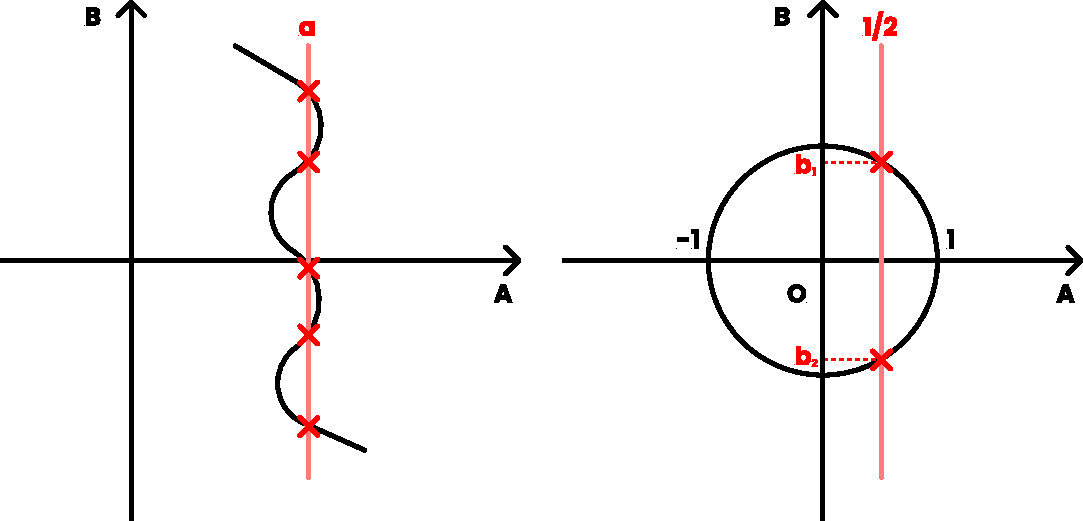
\includegraphics[width=10cm]{./images/notApplication.pdf}
\end{figure}

\noindent Un esempio di applicazione è invece:

\begin{figure}[h!]
    \centering
    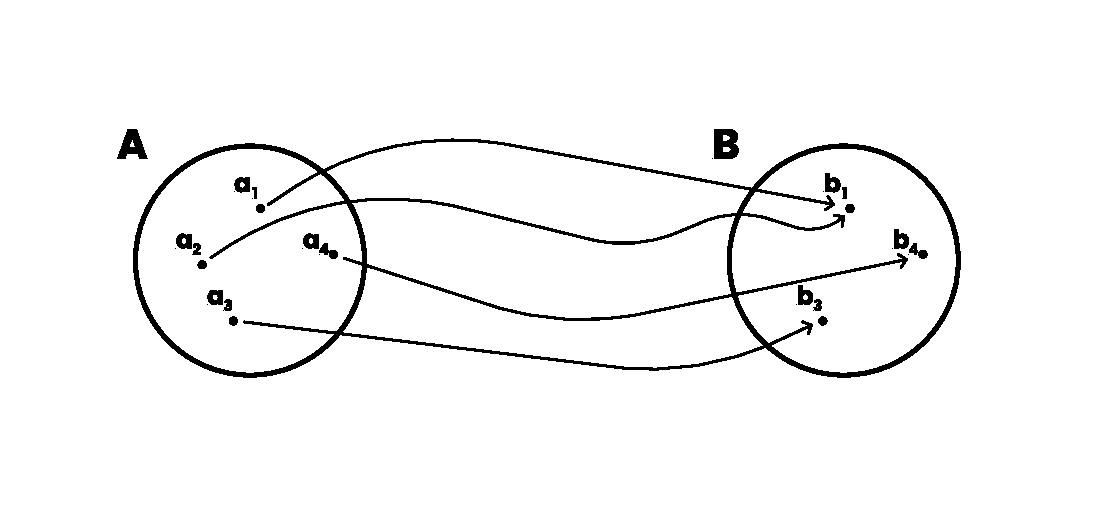
\includegraphics[width=11cm]{./images/application.pdf}
\end{figure}

\noindent Un'applicazione è formata da tre parti: due insiemi $A, B$ e una legge. Ad esempio: $\varphi: A \xrightarrow{} B$, è l'applicazione "phi" da $A$ a $B$, che ha come legge: $a \longmapsto \varphi(a) \ (\in B)$.\\

\noindent \textbf{Def:} $A = D(\varphi)$ è il dominio di $\varphi$, mentre $B = C(\varphi)$ è il codominio di $\varphi$.\\

\noindent \textbf{ES.} Le seguenti applicazioni sono tutte diverse, avendo insiemi diversi: 

\begin{equation*}
    f: \mathbb{R} \xrightarrow{} \mathbb{R} \quad x \longmapsto x^2 \qquad g: \mathbb{R} \xrightarrow{} [0, +\infty) \quad x \longmapsto x^2 \qquad h: [0, +\infty) \xrightarrow{} [0, +\infty) \quad x \longmapsto x^2
\end{equation*}

\noindent \textbf{Def:} L'\textbf{insieme immagine} di $\varphi$ è: $Imm(\varphi) = \{ b \in B \ | \ \exists a \in A \ per \ cui \ \varphi(a) = b \}$. Capiamo quindi che $Imm(\varphi) \subset B$. Un altro modo di scrivere questo insieme è: $Imm(\varphi) = \varphi(A)$. \\

\noindent Prendendo, ad esempio, l'applicazione $f$ scritta precedentemente, si può intuire che $Imm(f) = [0, +\infty)$, mentre $B = \mathbb{R}$, quindi $Imm(f) \subset B$. \\

\noindent \textbf{Def:} Sia $S \subset B$. Definisco controimmagine di $S$, secondo $\varphi$, l'insieme: 

\begin{equation*}
    \varphi^{-1} \vcentcolon = \{ a \in A \ | \ \varphi(a) \in S \} 
\end{equation*}

\noindent \textbf{NB!} $\varphi^{-1}$ non è il reciproco!\\

\noindent Presa, ad esempio, l'applicazione $f$ vista prima, possiamo capire che $\varphi(\{-1\})^{-1} = \varnothing$ (perché $x^2 \neq -1 \quad \forall x \in \mathbb{R}$) oppure $\varphi(\{1\})^{-1} = \{-1, 1\}$ (perché sia $x = -1$, che $x = 1$ elevati al quadrato mi danno $1$ come risultato). \\

\noindent \textbf{NB!} Dire $\{1, -1\}$ è diverso da dire $\{\pm 1\}$. Scrivere sempre e solo nel primo modo!

\subsection{Applicazione suriettiva, iniettiva e biettiva}
\textbf{Def:} Sia $\varphi: A \xrightarrow{} B$. Diremo che $\varphi$ è \textbf{suriettiva} se e solo se $Imm(f) = B$. Nell'esempio di prima, $f$ non è suriettiva, mentre $g$ e $h$ lo sono.\\

\noindent\textbf{Def:} Sia $\varphi: A \xrightarrow{} B$. Diremo che $\varphi$ è \textbf{iniettiva} se e solo se:

\begin{equation}
    \forall a_1, a_2 \in A \ con \ a_1 \neq a_2, \ si \ ha \ che \ \varphi(a_1) \neq \varphi(a_2)
    \label{eq:7}
\end{equation}

\noindent Equivalentemente, si può scrivere che: 

\begin{equation}
    \forall a_1, a_2 \in A \ | \ \varphi(a_1) = \varphi(a_2) \ si \ ha \ che \ a_1 = a_2
    \label{eq:8}
\end{equation}

\noindent Non è complicato dimostrare l'equivalenza di queste due definizioni. Basterà infatti procedere con una dimostrazione per contraddizione, che separi implicazione da controimplicazione. Partiamo quindi dall'implicazione ($\Rightarrow$), ovvero dalla definizione (\ref{eq:7}). Come ipotesi abbiamo che $a_1 \neq a_2$, mentre la tesi è che $\varphi(a_1) \neq \varphi(a_2)$. Negando quest'ultima (ovvero $\varphi(a_1) = \varphi(a_2)$), per la definizione di applicazione iniettiva, si ha che $a_1 = a_2$, che va però contro l'ipotesi iniziale. Arriviamo quindi ad una contraddizione. Ciò significa che se $a_1 \neq a_2$, allora per forza si ha che $\varphi(a_1) \neq \varphi(a_2)$. \\
Procediamo ora a verificare la controimplicazione ($\Leftarrow$; (\ref{eq:8})). L'ipotesi e la tesi sono rispettivamente $\varphi(a_1) = \varphi(a_2)$ e $a_1 = a_2$. Negando la tesi ($a_1 \neq a_2$), per definizione, abbiamo che $\varphi(a_1) \neq \varphi(a_2)$, il che va contro l'ipotesi iniziale. Per cui se $\varphi(a_1) = \varphi(a_2)$, allora per forza si ha che $a_1 = a_2$. \\

\noindent\textbf{Osservazione:} Sia $\varphi: A \xrightarrow{} B$:

\begin{enumerate}[label=\roman*)]
    \item $\varphi$ è suriettiva $\iff \forall b \in B, \exists a \in A \ | \ \varphi(a) = b$ (quindi $B \subseteq Imm(\varphi)$). Dato che per definizione $Imm(\varphi) \subseteq B \implies B = Imm(\varphi)$;
    \item $\forall b \in B, \exists !  a \in A \ | \ \varphi(a) = b$ (cioè ad ogni elemento del dominio corrisponde uno ed un solo elemento del codominio). In altre parole, è vero sia che $\varphi$ è suriettiva, sia che è iniettiva. Viene quindi detta \textbf{biettiva} o \textbf{biiezione} o \textbf{corrispondenza biunivoca}.
\end{enumerate}

\noindent Ritorniamo quindi un attimo agli esempi $f, g, h$. Consideriamo $f$: di certo non è suriettiva perché, ad esempio, $-1 \notin Imm(f)$. Ma è iniettiva? No, perché, ad esempio, $(1)^2 = 1$ e $(-1)^2 = 1$ (ci sono due punti distinti del dominio con la stessa immagine). \\
L'applicazione $g$, invece, è suriettiva ($Imm(g) = B$), ma non è iniettiva perché $\forall \alpha > 0, g^{-1}(\{\alpha\}) = \{-\sqrt{\alpha}, \sqrt{\alpha}\}$.\\
Infine, $h$ è sia suriettiva, sia iniettiva infatti $\forall \alpha > 0, g^{-1}(\{\alpha\}) = \{\sqrt{\alpha}\}$. Proprio per questo motivo, $h$ è biettiva.

\subsubsection{Corrispondenza biunivoca tra l'insieme dei numeri pari ed $\mathbb{N}$}
Siano $P = \{2m \ | \ m \in \mathbb{N}\}$ e $\mathbb{N}$. La nostra tesi è che esiste una corrispondenza biunivoca tra i due insiemi, in simboli:

\begin{equation*}
    P \overset{\Psi}{\longrightarrow} \mathbb{N}
\end{equation*}

\noindent\textbf{NB!} Cantor ha dimostrato che gli insiemi $\mathbb{N}, \mathbb{Z}, \mathbb{Q}$ sono tali che si può costruire tra loro una corrispondenza biunivoca. Sono infatti degli \textbf{insiemi numerabili}. Al contrario, $\mathbb{R}$ e $\mathbb{C}$ non sono numerabili.\\

\noindent Consideriamo quindi la seguente applicazione come biettiva: 

\begin{equation*}
    \Psi: \mathbb{N} \xrightarrow{} P \qquad m \longmapsto 2m \qquad \qquad con \ P \subsetneq \mathbb{N}
\end{equation*}

\noindent\textbf{Suriettività:} Sia $2m \in P$, la nostra tesi è che $\exists n \in \mathbb{N} \ | \ \Psi(n) = 2m$. Per definizione $\Psi(m) = 2m$, ma dato che dalla riga precedente abbiamo detto che $\Psi(n) = 2m$, allora $n = m$. Per questo motivo, $\Psi$ è suriettiva.\\

\noindent\textbf{Iniettività:} Siano $m_1 \neq m_2$ con $m_1, m_2 \in \mathbb{N}$. La nostra tesi è che $\Psi(m_1) \neq \Psi(m_2)$, dimostriamola per contraddizione! Supponiamo quindi che $\Psi(m_1) = \Psi(m_2)$. Ciò significa che se $\Psi(m_1) = 2m_1$ e $\Psi(m_2) = 2m_2$, allora $2m_1 = 2m_2$. Svolgendo un po' di conti:

\begin{equation*}
    2m_1 - 2m_2 = 0 \implies 2(m_1-m_2) = 0 \implies m_1 - m_2 = 0 \implies m_1 = m_2
\end{equation*}

\noindent Arriviamo quindi proprio ad una contraddizione, dato che per ipotesi $m_1 \neq m_2$, ne deriva che $\Psi(m_1) \neq \Psi(m_2)$. Quindi $\Psi$ è iniettiva.

\subsubsection{Paradosso del Grand Hotel di Hilbert}
Hilbert immagina un hotel con infinite stanze, tutte occupate, e afferma che qualsiasi sia il numero di altri ospiti che sopraggiungano, sarà sempre possibile ospitarli tutti, anche se il loro numero è infinito, purché numerabile.\\
Infatti, quando arrivano infiniti nuovi ospiti basta spostare ogni ospite nella stanza con numero doppio rispetto a quello attuale, lasciando così ai nuovi ospiti tutte le camere con i numeri dispari, che sono essi stessi infiniti, risolvendo dunque il problema. Gli ospiti sono tutti dunque sistemati, benché l'albergo fosse pieno.

\subsection{Somma, prodotto, rapporto e composizione di applicazioni}
\textbf{Def:} $\varphi: A \xrightarrow{} \mathbb{R}, \Psi: B \xrightarrow{} \mathbb{R}$, definiamo l'applicazione somma di $\varphi + \Psi$: 

\begin{equation*}
    (\varphi + \Psi): A \cap B \xrightarrow{} \mathbb{R} \qquad a \longmapsto \varphi(a) + \Psi(a)
\end{equation*}

\noindent Dato che il dominio è $A \cap B$, si capisce che nella somma, l'elemento $a$ deve appartenere sia ad $A$, che a $B$. \\

\noindent Dato che la somma in $\mathbb{R}$ è commutativa, allora: $(\varphi + \Psi) = (\Psi + \varphi)$ perché $\varphi(a) + \Psi(a) = \Psi(a) + \Psi(a)$.\\

\noindent\textbf{ES.} Dati $\varphi: [0, + \infty) \xrightarrow{} \mathbb{R} \quad x \longmapsto \sqrt{x}$ e $\Psi: \mathbb{R} \xrightarrow{} \mathbb{R} \quad x \longmapsto 2x$, allora $\varphi + \Psi: x \longmapsto \sqrt{x} + 2x \quad D(\varphi + \Psi) = [0, +\infty) \cap \mathbb{R} = [0, +\infty)$. \\

\noindent\textbf{Def:} Chiamiamo \textbf{grafico} di $\varphi: A \xrightarrow{} B$, l'insieme:
\begin{equation*}
    \Gamma(\varphi) = \mathcal{G}(\varphi) = \{(a, \varphi(a)) \ | \ a \in A\} \quad dove \ \varphi(a) \in B
\end{equation*}

\noindent\textbf{NB!} $\Gamma(\varphi) = \mathcal{G}(\varphi)$ è un sottoinsieme del prodotto cartesiano $C(A\times B)$. \\

\noindent Sia $f: A \xrightarrow{} \mathbb{R}$ e $c: \mathbb{R} \xrightarrow{} \mathbb{R} \quad x \longmapsto c$. \\
\noindent Prendiamo ora $D(f + c) = D(f) \cap D(c) = A \cap \mathbb{R} = A$. \\
\noindent Possiamo capire semplicemente che preso il grafico di $f$ e quello di $f + c$, essi variano solo per la seconda componente:
\begin{gather*}
    \mathcal{G}(f + c) = \{(a, f(a) + c) \ | \ a \in A\}\\
    \mathcal{G}(f) = \{(a, f(a)) \ | \ a \in A\}
\end{gather*}

\noindent Questa componente $c$ permette di traslare il grafico. In particolare:

\begin{itemize}
    \item se $c > 0$, allora $f(a) < f(a) + c$ e quindi l'applicazione trasla rigidamente verso l'alto;
    \item se $c < 0$, allora $f(a) > f(a) + c$ e quindi l'applicazione trasla rigidamente verso il basso.
\end{itemize}

\noindent\textbf{NB!} $c: \mathbb{R} \xrightarrow{} \mathbb{R} \quad x \longmapsto c$ viene definita \textbf{applicazione costante} perché va da $\mathbb{R} \xrightarrow{} \mathbb{R}$ e ad ogni $x$ associa lo stesso valore $c$. Per questo motivo, non è né iniettiva (perché ogni punto di $\mathbb{R}$ finisce nella stessa immagine), né suriettiva (perché l'immagine è solo $c$, mentre il codominio è tutto $\mathbb{R}$).\\

\noindent Sia $f: D(f) \xrightarrow{} \mathbb{R} \quad x \longmapsto f(x)$, allora se prendiamo $\mathcal{G}(bf): (bf): D(f) \xrightarrow{} \mathbb{R} \quad x \longmapsto bf(x) \quad con \ b \in \mathbb{R}$, esso dipenderà proprio da $b$. In particolare: 

\begin{itemize}
    \item se $b = 1$, ovviamente il grafico rimane uguale;
    \item se $b > 0 \wedge b \neq 1$, viene applicato un effetto di \textbf{deformazione} all'applicazione;
    \item se $b = -1$ il grafico viene \textbf{ribaltato};
    \item se $b < 0 \wedge b \neq -1$, viene applicato un effetto di \textbf{deformazione} all'applicazione dovuto a $|b|$ ed un effetto di \textbf{ribaltamento} dovuto al fatto che $b < 0$.
\end{itemize}

\noindent Sia ora $f: A \subset \mathbb{R} \xrightarrow{} \mathbb{R} \quad x \longmapsto f(x)$ e $g: C \subset \mathbb{R} \xrightarrow{} \mathbb{R} \quad x \longmapsto f(x + c)$, dove $c \in \mathbb{R}$ ed è fissato. Notiamo che in $g$ stanno avvenendo due operazioni: prima trasliamo $x$ in $x + c$ e poi applichiamo il risultato ad $f$. Il dominio di $g$ sarà quindi: $C = D(g) = \{x \in \mathbb{R} \ | \ (x + c) \in D(f) = A\}$. Ciò significa quindi che $x+c = a$ dove $a \in A$. In particolare, si ha che $A = \{x \in \mathbb{R} \ | \ \exists a \in A \ tale \ che \ x = a -c\}$. In altre parole, stiamo traslando il dominio $D(f)$ di una certa quantità $c$. \\

\noindent\textbf{ES.} Sia $A = [-1, 1] \quad c = 2$, allora $C = \{x \in \mathbb{R} \ | \ \exists a \in [-1, 1] \ tale \  che \ x = a-2\}$. Quindi $C = [-3, -1]$.\\

\noindent\textbf{NB!} A volte si trova anche la notazione $C = \{a-b \ | \ a \in A, b \in B\} = \vcentcolon A - B$, dove, secondo l'esempio di prima, $B = \{c\}$.\\

\noindent\textbf{Def:} Dati $A, B$ con $A \cap B \neq \varnothing$. Siano $\varphi: A \xrightarrow{} \mathbb{R}$ e $\Psi: B \xrightarrow{} \mathbb{R}$. L'applicazione prodotto è:
\begin{gather*}
    \Psi \cdot \varphi: (A \cap B) \xrightarrow{} \mathbb{R}\\
    a \longmapsto \Psi(a) \cdot \varphi(a)
\end{gather*}

\noindent Come nel caso della somma tra due applicazioni, si ha che $\Psi \cdot \varphi = \varphi \cdot \Psi$ perché il prodotto $\Psi(a) \cdot \varphi(a) = \varphi(a) \cdot \Psi(a)$.\\

\noindent\textbf{Def:} Dati $A, B$ con $A \cap B \neq \varnothing$. Siano $\varphi: A \xrightarrow{} \mathbb{R}$ e $\Psi: B \xrightarrow{} \mathbb{R}$. L'applicazione rapporto è:
\begin{gather*}
    \frac{\Psi}{\varphi}: (A \cap B) \cap \{a \in A \ | \ \varphi(a) \neq 0 \} \xrightarrow{} \mathbb{R} \\
    a \longmapsto \frac{\Psi(a)}{\varphi(a)}
\end{gather*}

\noindent\textbf{NB!} La condizione aggiunta rispetto alla somma e al prodotto serve a specificare che il denominatore dev'essere non nullo. \\

\noindent\textbf{NB!} Definiamo l'insieme degli zeri di un'applicazione $f$: $z_f = \{a \in D(f) \ | \ f(a) = 0\}$. Allora dire che $\dfrac{\Psi}{\raisebox{0.2ex}{$\varphi$}} \neq \dfrac{\raisebox{0.4ex}{$\varphi$}}{\raisebox{-0.3ex}{$\Psi$}}$, infatti:

\begin{equation*}
    D\left(\frac{\Psi}{\varphi}\right) - z_\varphi \quad D\left(\frac{\raisebox{0.4ex}{$\varphi$}}{\raisebox{-0.3ex}{$\Psi$}}\right) - z_\Psi \implies D\left(\frac{\Psi}{\varphi}\right) \neq D\left(\frac{\raisebox{0.4ex}{$\varphi$}}{\raisebox{-0.3ex}{$\Psi$}}\right)
\end{equation*}

\section{Topologia della retta reale}
\textbf{Def:} Sia $x \in \mathbb{R}$ e sia $\varepsilon > 0$. Diremo \textbf{intorno} di centro $x_0$ e raggio $\delta$ l'intervallo: 

\begin{equation*}
    D(x_0, \delta) \vcentcolon = \{x\in\mathbb{R} \ | \ |x - x_0| < \delta\} \vcentcolon = (x_0 - \delta, x_0 + \delta)
\end{equation*}

\noindent\textbf{NB!} Viene anche detto \textbf{intorno circolare}.\\

\noindent\textbf{Intorno di $+\infty$ - Def:}  Ogni intervallo del tipo $(a, + \infty)$ per $a \in \mathbb{R}$:

\begin{equation*}
    \{x\in\mathbb{R} \ | \ x > a\}
\end{equation*}

\noindent ovvero tutti gli intervalli non superiormente limitati.\\

\noindent\textbf{Intorno di $-\infty$ - Def:}  Ogni intervallo del tipo $(- \infty, a)$ per $a \in \mathbb{R}$:

\begin{equation*}
    \{x\in\mathbb{R} \ | \ x < a\}
\end{equation*}

\noindent È facile capire quindi che in questi insiemi si ha:
\begin{gather*}
    sup((a, +\infty)) = +\infty \qquad inf((a, +\infty)) = a \\
    sup((-\infty, a)) = a \qquad inf((-\infty, a)) = - \infty
\end{gather*}

\noindent Prima di continuare con la spiegazione, definiamo l'insieme $\widetilde{\mathbb{R}} = \mathbb{R} \cup \{-\infty, +\infty\}$, dove $\widetilde{\mathbb{R}}$ si legge \textbf{$\mathbb{R}$ esteso}. In altre parole, se $x_0 \in \widetilde{\mathbb{R}}$, allora o $x_0 \in \mathbb{R}$ o $x_0 = +\infty$ oppure $x_0 = - \infty$.\\

\noindent \textbf{Def:} Sia $A \subset \mathbb{R}$ con $A \neq \varnothing$. Sia ora $x_0 \in \mathbb{R}$. Diremo che $x_0$ è \textbf{punto di accumulazione} per $A$ se e solo se:

\begin{equation*}
    \forall \delta > 0 \ si \ ha \ che \ (D(x_0, \delta) \cap A) - \{x_0\} \neq \varnothing
\end{equation*}

\noindent In altre parole, significa che esistono punti di $A$, diversi da $x_0$, arbitrariamente vicini a $x_0$. \\

\noindent\textbf{NB!} $D(x_0, \delta)$ è un intorno circolare di $x_0$.\\

\noindent\textbf{NB!} $x_0 \in \mathbb{R}$, ma non deve per forza appartenere ad $A$ per essere un suo punto di accumulazione.

\subsection{Esercizio 5}
\textbf{Sia $A = (1, 2) \cup \{3\}$. Quali sono i punti di accumulazione reali di $A$?}

\noindent Ipotizziamo che $x < 1$. Prendendo quindi un $\delta > 0$, otteniamo un intorno $I = (x - \delta, x + \delta) \cap A$. In particolare, questo intorno $I$ sarà composto da tutti i numeri compresi tra $1$ e $x + \delta$. Questo però non vale per ogni $\delta > 0$. Infatti, se prendiamo $\delta < \Delta = 1 - x$ (dove $\Delta$ rappresenta la distanza tra $1$ e $x$), si ha che $I = \varnothing$. Ciò significa che se $x < 1$, allora $x$ non è un punto di accumulazione. 
Si può anche osservare quanto spiegato qui sopra dalla prima immagine della prossima pagina.

\noindent Sia ora $x = 1$ (come detto precedentemente, anche se $1 \notin A$, non significa che esso non possa essere punto di accumulazione per $A$). Allora possiamo prendere un $\delta > 0$, tale che $J = (1 - \delta, 1 + \delta) \cap A \neq \varnothing$. Dato che quest'ultima relazione deve essere verificata per ogni $\delta > 0$, dobbiamo procedere con tutti i casi. Di seguito, troviamo le immagini raffiguranti cosa succede in ogni caso e un sistema finale che riassume tutti i conti.

\begin{figure}[!h]
    \centering
    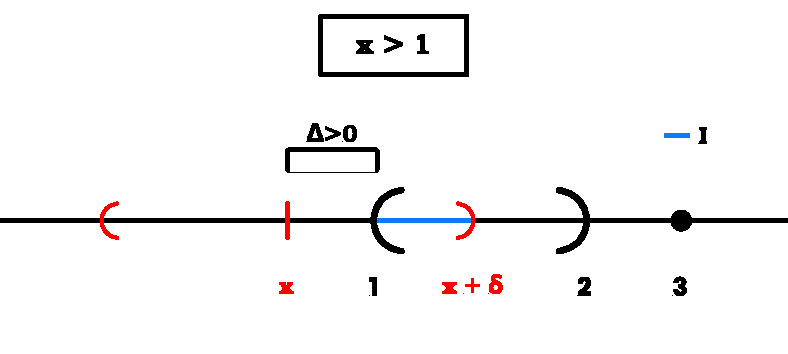
\includegraphics[width=12cm]{./images/AccPoints1.pdf}
\end{figure}

\begin{figure}[!h]
    \centering
    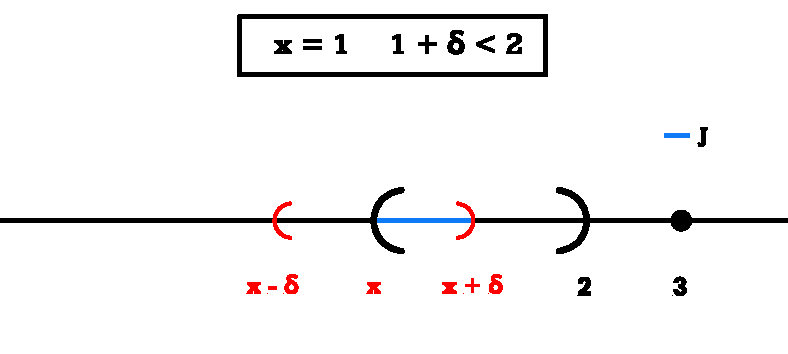
\includegraphics[width=7cm]{./images/AccPoints2.pdf}\hfill
    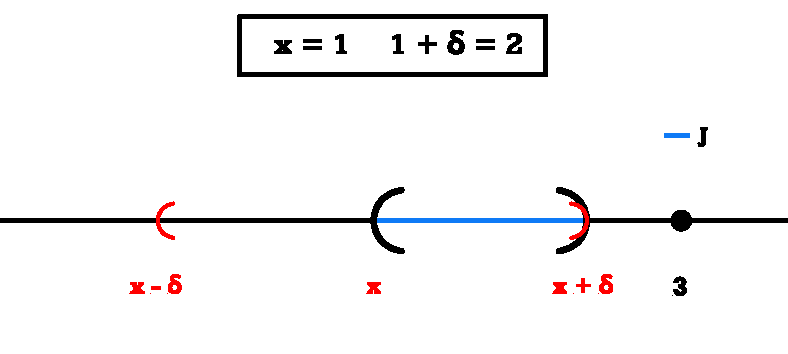
\includegraphics[width=7cm]{./images/AccPoints3.pdf}
\end{figure}

\begin{figure}[!h]
    \centering
    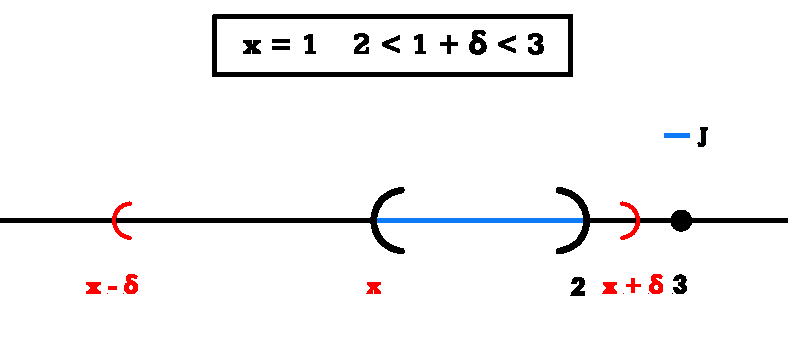
\includegraphics[width=7cm]{./images/AccPoints4.pdf}\hfill
    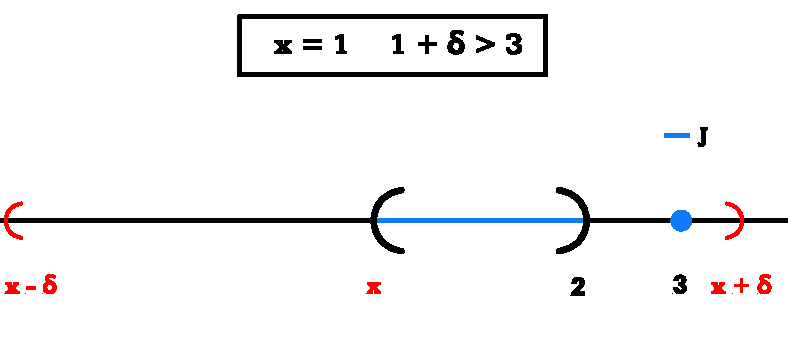
\includegraphics[width=7cm]{./images/AccPoints5.pdf}
\end{figure}

\begin{equation*}
    J =
    \begin{cases}
    (1, 1 + \delta) \quad se \ \delta < 1 \\
    (1, 2) \quad se \ \delta = 1 \\
    (1, 2) \quad se \ 1 < \delta < 2 \\
    (1, 2) \quad se \ \delta = 2 \\
    A \quad se \ \delta > 2
\end{cases}
\end{equation*}

\noindent Dato che per la definizione di punto di accumulazione, dall'intersezione $D(x_0,\delta) \cap A$ è necessario togliere $x_0$, togliendo $x = 1$ da $J$, notiamo che esso rimane non vuoto. Possiamo quindi concludere che $1$ è punto di accumulazione per l'insieme $A$.

\subsection{Esercizio 6}
\textbf{Verificare che $x = 2$ è punto di accumulazione.}

\noindent Procediamo allo stesso modo di prima:

\begin{equation*}
    J = \begin{cases}
        A \quad se \ 2 - \delta < 1 \implies \delta > 1 \\
        (2-\delta, 2) \quad se \ 2 - \delta > 1 \implies \delta < 1 \\
        A \quad se \ \delta = 1
    \end{cases}
\end{equation*}

\noindent In generale, togliendo $x = 2$ da $J$ notiamo che esso rimane non vuoto. Possiamo quindi concludere che $2$ è punto di accumulazione per l'insieme $A$. Di seguito, è possibile verificare graficamente perché abbiamo ottenuto questi risultati. 

\begin{figure}[!h]
    \centering
    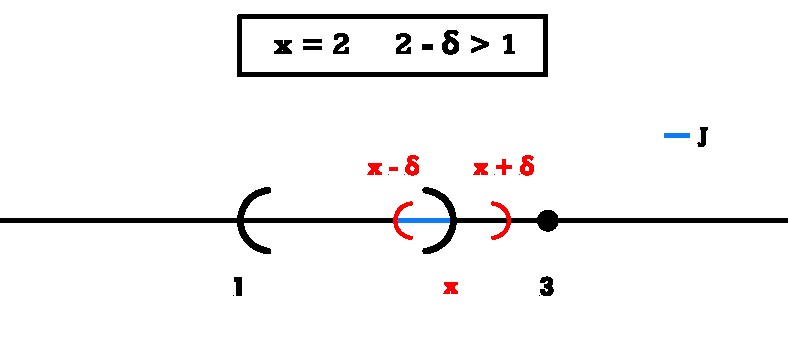
\includegraphics[width=7cm]{./images/AccPoints6.pdf}\hfill
    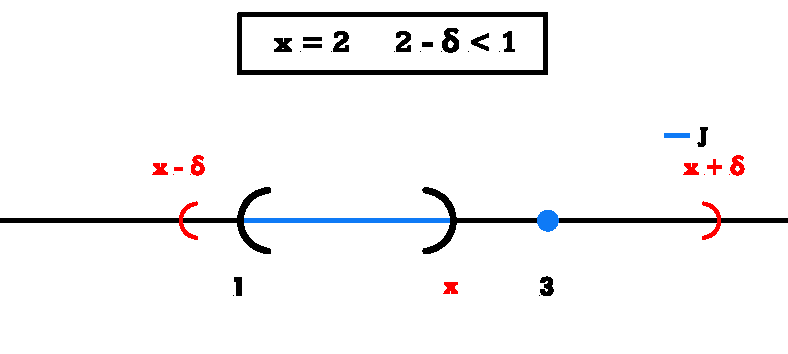
\includegraphics[width=7cm]{./images/AccPoints7.pdf}
\end{figure}

\begin{figure}[!h]
    \centering
    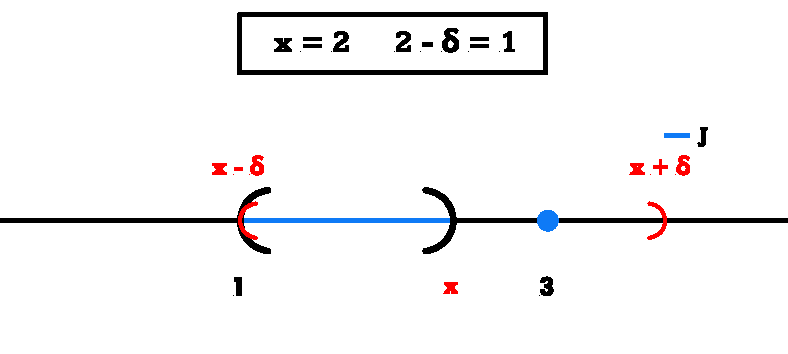
\includegraphics[width=12cm]{./images/AccPoints8.pdf}
\end{figure}

\subsection{Esercizio 7}
\textbf{Verificare che qualsiasi $x_0 \in (1, 2)$ è punto di accumulazione per $A$.}

\noindent Semplicemente, essendo $x_0 \in (1, 2)$, ciò significa che $1 < x_0 < 2$. A livello visivo:

\begin{figure}[!h]
    \centering
    $\vcenter{\hbox{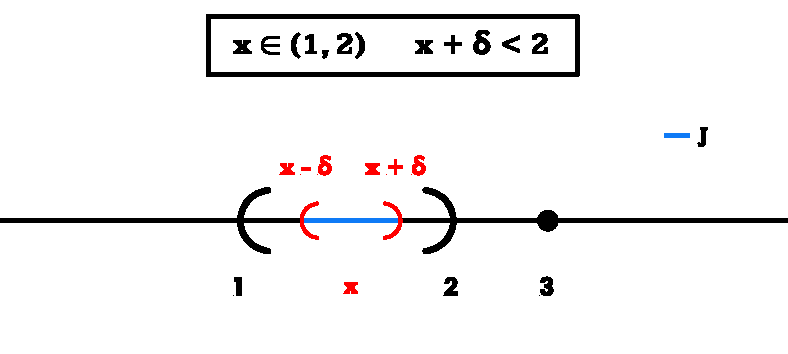
\includegraphics[width=5cm]{./images/AccPoints9.pdf}}}$\hfill
    $\vcenter{\hbox{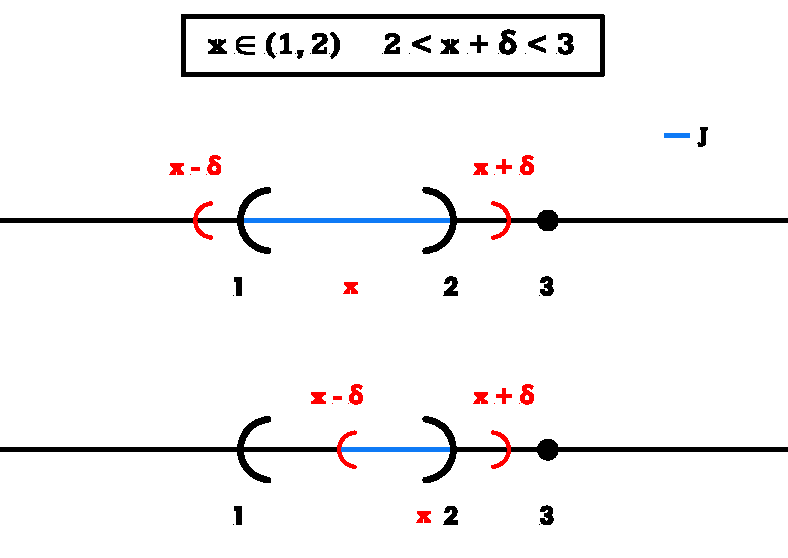
\includegraphics[width=5cm]{./images/AccPoints10.pdf}}}$\hfill
    $\vcenter{\hbox{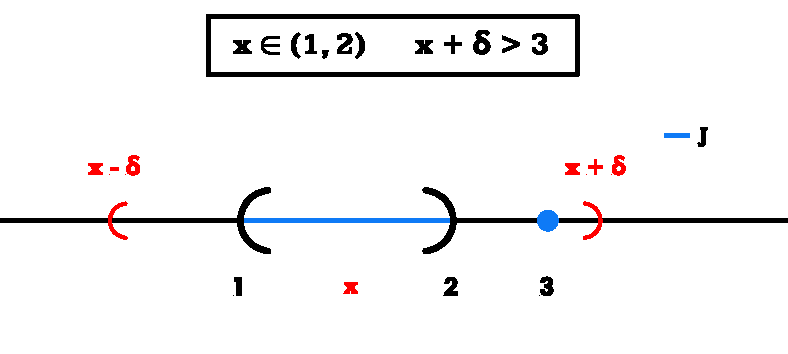
\includegraphics[width=5cm]{./images/AccPoints11.pdf}}}$
\end{figure}

\noindent Quindi:

\begin{itemize}
    \item se $x_0 + \delta < 2$, allora $J = (x_0 - \delta, x_0 + \delta)$;
    \item se $2 < x_0 + \delta < 3$, allora:
    \begin{itemize}
        \item se $x_0 - \delta > 1$, allora $J = (x_0 - \delta, 2)$;
        \item se $x_0 - \delta < 1$, allora $J = (1, 2)$
    \end{itemize}
    \item se $x_0 + \delta > 3$, allora $J = A$;
    \item se $x_0 + \delta = 2$, allora:
    \begin{itemize}
        \item se $x_0 - \delta \leq 1$, allora $J = (1, 2)$;
        \item se $x_0 - \delta > 1$, allora $J = (x_0 - \delta, 2)$.
    \end{itemize}
\end{itemize}

\noindent Togliendo ora $x_0$ da $J$, quest'ultimo rimane non vuoto. Per cui possiamo concludere che qualsiasi $x_0 \in (1, 2)$ è un punto di accumulazione.

\subsection{Esercizio 8}
\textbf{Verificare che qualsiasi $x > 2 \wedge x \neq 3$, $x$ non è punto di accumulazione per $A$.}

\noindent Per farlo basta trovare un unico caso per cui vale che $J = ((x_0 - \delta, x_0 + \delta) \cap A) - \{x_0\} = \varnothing$. Prendendo quindi $x_0 + \delta < 3$ oppure prendendo un numero $x > 3$ e un $\delta < \Delta = x - 3$ (dove $\Delta$ è la distanza tra $x$ e $3$), si ha che non vi è nessuna intersezione con l'insieme A e quindi $J = \varnothing$. Per cui possiamo concludere che $3$ non è un punto di accumulazione per $A$. Graficamente:

\begin{figure}[!h]
    \centering
    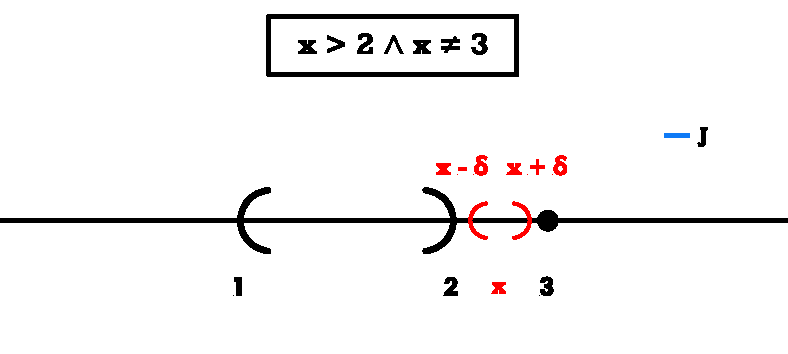
\includegraphics[width=12cm]{./images/AccPoints12.pdf}
\end{figure}

\subsection{Esercizio 9}
\textbf{Dimostrare che $x_0 = 3$ non è punto di accumulazione per $A$.}

\noindent Dire che $x_0 = 3$ non è punto di accumulazione per $A$, significa che $\exists \Bar{\delta} > 0 \ | \ ((3 - \Bar{\delta}, 3 + \Bar{\delta}) \cap A) - \{3\} = \varnothing$. \\
Se prendiamo un $\Bar{\delta} > 0$ tale che $3 - \Bar{\delta} > 2 \implies \Bar{\delta} < 1$ avremo che $((3 - \Bar{\delta}, 3 + \Bar{\delta}) \cap A) - \{3\} = \varnothing$. Si verifica infatti con, ad esempio, $\Bar{\delta} = \dfrac{1}{2}$. Per questo motivo, possiamo concludere che $3$ non è un punto di accumulazione per $A$.\\

\subsection{Esercizio 10}
\textbf{Sia $B = [1, 2] \cup \{3\}$, provare che i punti di accumulazione di $B$ sono tutti e soli quelli dell'insieme $[1,2]$.}

\noindent Procediamo per casi: 

\begin{itemize}
    \item Se $x < 1$, allora, come per il primo esempio su questa tipologia di esercizi, $x$ non è punto di accumulazione perché preso un $\delta < \Delta = 1 - x$ (dove $\Delta$ rappresenta la distanza tra $1$ e $x$), l'intersezione $J = \varnothing$;
    \item se $x = 1$, allora:
    \begin{itemize}
        \item se $1 < 1 + \delta < 2 \implies 0 < \delta < 1$, avremo che $J = [1, x_0 + \delta)$;
        \item se $1 + \delta > 2 \implies \delta > 1$, avremo che $J = [1, 2]$;
        \item se $1 + \delta = 2 \implies \delta = 1$, avremo che $J = [1, 2)$;
    \end{itemize}
    \item se $1 < x < 2$, allora:
    \begin{itemize}
        \item se $1 + \delta < 2 \implies \delta < 1$, allora $J = (1 - \delta, 1 + \delta)$;
        \item se $1 + \delta = 2 \implies \delta = 1$, allora $J = (1 - \delta, 2)$;
        \item se $1 + \delta > 2 \implies \delta > 1$, allora:
        \begin{itemize}
            \item $x_0 - \delta > \Delta = x - 1$, allora $J = (x_0 - \delta, 2]$;
            \item se $x_0 - \delta < \Delta = x - 1$, allora $J = [1, 2]$;
            \item se $x_0 - \delta < \Delta = x - 1$, allora $J = (1, 2]$
        \end{itemize}
    \end{itemize}
    \item se $x = 2$, allora: 
    \begin{itemize}
        \item se $x_0 - \delta > 1$, allora $J = (x_0 - \delta, 2]$;
        \item se $x_0 - \delta < 1$, allora $J = A$;
        \item se $x_0 - \delta = 1$, allora $J = (1, 2]$;
    \end{itemize}
    \item se $x > 2$, allora, come per $x < 1$, preso $\delta > \Delta = x - 2$, allora $J = \varnothing$.
\end{itemize}

\noindent Notiamo come in tutti per qualsiasi $x$ tale che $x < 1$ o $x > 2$, essa non è punto di accumulazione di $a$, mentre $x \in [1, 2]$ è un punto di accumulazione, come volevasi dimostrare.\\

\subsection{Esercizio 11}
\textbf{Sia $I = (a, b)$, $J = [a, b)$, $K = (a, b]$ e $L = [a, b]$. Provare che i punti di accumulazione di $I, J, K, L$ sono tutti e soli i punti $[a, b]$.}

\noindent Ancora una volta procediamo per casi:

\begin{itemize}
    \item se $x < a$ e $\delta < \Delta = 1 - x$, allora qualsiasi sia l'insieme che stiamo valutando, esso sarà vuoto;
    \item se $x = a$, allora l'insieme derivante dall'intersezione sarà pari a $[a, x_0 + \delta)$ (oppure a $[a, b]$, se $x_0 + \delta > b$);
    \item se $a < x < b$, allora:
    \begin{itemize}
        \item se $x_0 + \delta < b$, allora:
        \begin{itemize}
            \item se $x_0 - \delta < a$, allora l'insieme derivante dall'intersezione sarà pari a $[a, x_0 + \delta)$;
            \item se $x_0 - \delta > a$, allora l'insieme derivante dall'intersezione sarà apri a $(x_0 - \delta, x_0 + \delta)$;
        \end{itemize}
        \item se $x_0 + \delta > b$, allora:
        \begin{itemize}
            \item se $x_0 - \delta < a$, allora l'insieme derivante dall'intersezione sarà pari a $[a, b]$;
            \item se $x_0 - \delta > a$, allora l'insieme derivante dall'intersezione sarà pari a $(x_0 - \delta, b]$;
        \end{itemize}
    \end{itemize}
    \item se $x = b$, allora l'insieme derivante dall'intersezione sarà pari a $(x_0 + \delta, b]$ (oppure a $[a, b]$, se $x_0 - \delta < a$);
    \item se $x > b$, allora basterà prendere un $\delta > \Delta = x - b$ per far in modo che qualsiasi sia l'insieme considerato, l'intersezione prodotta sia un insieme vuoto.
\end{itemize}

\noindent Notiamo quindi che tutti i valori di $x < a \vee x > b$ non sono punti di accumulazione perché l'intersezione prodotta è pari ad un insieme vuoto; mentre i punti $a \leq x \leq b$ sono tutti punti di accumulazione per qualsiasi dei quattro insiemi considerati (a seconda dell'insieme considerato, le parentesi quadre della lista qui sopra potrebbero essere delle parentesi tonde).\\

\noindent\textbf{Def:} Chiamiamo \textbf{punti isolati} i punti $x_0 \in \mathbb{R}$ dell'insieme $A \subset \mathbb{R}$ con $A \neq \varnothing$ se e solo se $x_0$ \textbf{non} è un punto di accumulazione. Un punto, quindi, può appartenere ad un insieme, ma allo stesso tempo essere isolato. \\

\noindent\textbf{Def:} $+ \infty$ è un punto di accumulazione per $A \subset \mathbb{R}$ con $A \neq \varnothing$ se e solo se ogni intorno di $+ \infty$ contiene punti di $A$. Scritto in simboli:

\begin{equation*}
    \forall b \in \mathbb{R} \ si \ ha \ che \ (A \cap (b, + \infty) \neq \varnothing)
\end{equation*}

\noindent\textbf{NB!} Nel caso del $+\infty$ o del $-\infty$ non va tolto il numero stesso (infatti nella formula non è presente il $- \{x_0\}$).\\

\noindent\textbf{NB!} Ciò significa che nell'insieme $A$ ci sono numeri arbitrariamente grandi.\\

\noindent\textbf{Def:} $- \infty$ è un punto di accumulazione per $A \subset \mathbb{R}$ con $A \neq \varnothing$ se e solo se:

\begin{equation*}
    \forall b \in \mathbb{R} \ si \ ha \ che \ (A \cap (- \infty, b) \neq \varnothing)
\end{equation*}

\noindent\textbf{Osservazione:} Se $A$ è superiormente limitato (inferiormente limitato) è possibile che $+ \infty$ ($- \infty$) sia punto di accumulazione per $A$? No, perché se $A$ è superiormente limitato (inferiormente limitato), allora $A$ ammette maggioranti (minoranti). Sia $\Lambda$ maggiorante (minorante) di $A$, cioè $\Lambda \in \mathbb{R}, a \leq \Lambda \quad \forall a \in A$ ($\Lambda \in \mathbb{R}, \Lambda \leq a \quad \forall a \in A$). Allora $A \subset (- \infty, \Lambda)$ ($A \subset (\Lambda, + \infty)$) e se $b = \Lambda + 1$ ($b = \Lambda - 1$), allora $A \cap (\Lambda + 1, +\infty) = \varnothing$ ($A \cap (-\infty, \Lambda - 1) = \varnothing$).\\

\noindent\textbf{Def:} Sia $f: A \subset \mathbb{R} \xrightarrow{} \mathbb{R}$ con $A \neq \varnothing$. Sia $x_0 \in \widetilde{\mathbb{R}}$ un punto di accumulazione per $A$. Diremo che $f$ ammette limite $l \in \widetilde{\mathbb{R}}$ per $x$ che tende a $x_0$ e scriveremo  $$\lim_{x \to x_0} f(x) = l$$ se e solo se per ogni intorno $V_l$ di $l$, esiste un intorno $U_{x_0}$ (intorno di $x_0$) tale che $$f(x) \in V_l \quad \forall x \in (U_{x_0} \cap A) - \{x_0\}$$

\noindent\textbf{NB!} È bene specificare che $x_0$ è un punto di accumulazione, altrimenti l'insieme qui sopra potrebbe essere un insieme vuoto $\varnothing$. Proprio per questo motivo, prima di risolvere un limite è bene sempre verificare che $x_0$, ovvero il punto a cui si sta tendendo, sia sempre un punto di accumulazione, altrimenti il limite non esiste.\\

\noindent\textbf{NB!} $U_{x_0}$ dipende da $l$. Più nello specifico, esso dipende da $V_l$, l'intorno di $l$. Quindi se cambio $V_l$, allora cambio anche $U_{x_0}$. \\

\noindent\textbf{NB!} Se $x_0 \in \{-\infty, + \infty\}$, l'ultima intersezione è da leggere come $U_{x_0} \cap A$ (ovvero senza togliere $\{x_0\}$).\\

\noindent\textbf{ES.} Se $l \in \mathbb{R}$ e $x_0 \in \mathbb{R}$, allora $V_l = (l - \varepsilon, l + \varepsilon) \quad \forall \varepsilon > 0$ e $U_{x_0} = (x_0 - \delta_\varepsilon, x_0 + \delta_\varepsilon)$.

\begin{equation*}
    \implies \forall \varepsilon > 0, \exists \delta_\varepsilon > 0 \ : \ | f(x) - l | < \varepsilon \qquad \forall x \in A, 0 < | x - x_0 | < \delta_\varepsilon
\end{equation*}

\noindent\textbf{NB!} Dire che $| f(x) - l | < \varepsilon$, significa dire che $f(x) \in V_l$. Mentre dire che $| x - x_0 | < \delta_\varepsilon$, significa dire che $x_0 \in (U_{x_0} \cap A)$. Perché invece è presente $0 < | x - x_0 |$? In generale, se $|u| \geq 0$, si ha che $|u| = 0 \iff u = 0$. Quindi mettere il maggiore stretto di $0$, significa che non si presenterà mai il caso in cui $x - x_0 = 0$, ovvero il caso in cui $x = x_0$. In altre parole, si verifica sempre il caso di $x \neq x_0$.\\

\noindent\textbf{NB!} Quando si parla di \textbf{disco bucato in $x_0$}, significa che è stato preso un disco centrato in $x_0$, ma è stato tolto $x_0$ stesso.\\

\noindent\textbf{ES.} Se invece avessimo $l = + \infty$ e $x_0 \in \mathbb{R}$, allora $V_l = (M, + \infty) \quad \forall M > 0$ e $U_{x_0} = (x_0 - \delta, x_0 + \delta)$.

\begin{equation*}
    \implies \forall M > 0, \exists \delta > 0 : f(x) > M \qquad \forall x \in (x_0 - \delta, x_0 + \delta) \cap A - \{x_0\}
\end{equation*}

\noindent\textbf{NB!} Dire che $f(x) > M$, significa dire che $f(x) \in V_l$.

\subsection{Esercizio 12}
\textbf{Esiste il seguente limite?}

\begin{equation*}
    \lim_{x \to -\infty} \frac{2x-1}{\sqrt{x+2}}
\end{equation*}

\noindent Innanzitutto, troviamo il \textbf{campo di esistenza} (dominio) della funzione. Il numeratore è un semplice polinomio, che ha quindi dominio $\mathbb{R}$, mentre il denominatore, essendo una radice, ha come dominio il proprio argomento maggiore o uguale a zero. Dato però che si trova appunto al denominatore, dobbiamo escludere il caso in cui l'espressione si annulla. Facendo un po' di conti, troviamo quindi che il dominio è $x > -2 \implies (-2, + \infty)$.\\

\noindent Dato che $-\infty$ non è un punto di accumulazione (perché l'insieme è inferiormente limitato), il limite non esiste.

\subsection{Esercizio 13 - Non finito}
\textbf{È vero che:}

\begin{equation*}
    \lim_{x \to 2} \frac{2x-1}{x+2} = \frac{3}{4}
\end{equation*}

\noindent Innanzitutto, notiamo che il dominio della funzione risulta essere $x \neq -2 \implies A = \mathbb{R} - \{-2\} = (-\infty, -2) \cup (-2, + \infty) \neq \varnothing$.\\
Successivamente, ci chiediamo se $2$ è un punto di accumulazione. Guardando il dominio, capiamo subito che qualsiasi sia il $\delta > 0$ preso, l'intersezione tra campo di esistenza e intorno considerato produrrà sempre un insieme non vuoto. Infatti, se $2 - \delta > -2$, allora l'intorno $I = (2 - \delta, 2 + \delta)$; mentre se $2 - \delta < -2$, allora $I = (2-\delta, -2) \cup (-2, 2 + \delta$). \\
È possibile anche mostrare che i punti di accumulazione di $A$ sono dati da $\widetilde{\mathbb{R}}$. Infatti, $A$ non essendo limitato possiede come punti di accumulazione anche $+ \infty$ e $- \infty$, che appartengono proprio a $\widetilde{\mathbb{R}}$. Non ci resta che verificare che tutti i punti appartenenti ad $\mathbb{R}$ sono punti di accumulazione di $A$. Non è complicato notare però che sia che $x < -2$ o che $x > - 2$, qualsiasi sia $\delta > 0$, il nostro intorno $I$ starà sempre intersecando $A$ e quindi l'intersezione sarà un insieme non vuoto. Per cui possiamo concludere che i punti di accumulazione di $A$ sono dati da $\widetilde{\mathbb{R}}$.\\

\noindent Per verificare la definizione di limite:

\begin{equation*}
    \forall \varepsilon > 0, \exists \delta_\varepsilon > 0 \ : \ \left| \frac{2x-1}{x+1} - \frac{3}{4} \right| < \varepsilon \qquad \forall x \in A, x \in (2-\delta_\varepsilon, 2+\delta_\varepsilon) - \{2\} \neq \varnothing
\end{equation*}

\noindent ossia per $\varepsilon > 0$:

\begin{equation*}
    \left| \frac{2x-1}{x+1} - \frac{3}{4} \right| < \varepsilon \iff \frac{3}{4} - \varepsilon < \frac{2x - 1}{x + 2} < \frac{3}{4} + \varepsilon
\end{equation*}

\noindent Consideriamo ora il caso in cui $x + 2 > 0 \implies x > -2$, possiamo quindi moltiplicare a destra e a sinistra per $x + 2$, senza cambiare il segno della disequazione:

\begin{equation*}
    \left(\frac{3}{4} - \varepsilon\right)(x+2) < 2x - 1 < \left(\frac{3}{4} + \varepsilon\right)(x+2)
\end{equation*}

\noindent Dividiamo ora le due disequazioni in un sistema e svolgiamo i calcoli:

\begin{equation*}
    \begin{cases}
        2x < \dfrac{3}{4}x + \dfrac{3}{2} + \varepsilon x + 2\varepsilon + 1 \\
        \\
        2x > \dfrac{3}{4}x + \dfrac{3}{2} - \varepsilon x - 2\varepsilon + 1 \\
    \end{cases}
    \implies
    \begin{cases}
        x\left(2 - \dfrac{3}{4} - \varepsilon\right) < \dfrac{5}{2} + 2\varepsilon \\
        \\
        x\left(2 - \dfrac{3}{4} + \varepsilon \right)>  \dfrac{5}{2} - 2\varepsilon \\
    \end{cases}
    \implies
    \begin{cases}
        x\left(\dfrac{5 - 4\varepsilon}{4}\right) < \dfrac{5 + 4\varepsilon}{2}\\
        \\
        x\left(\dfrac{5 + 4\varepsilon}{4}\right)>  \dfrac{5 - 4\varepsilon}{2} \\
    \end{cases}
\end{equation*}

\noindent Consideriamo ora la prima disequazione. Si possono presentare due casi:

\begin{itemize}
    \item se $5 - 4\varepsilon > 0 \implies \varepsilon < \dfrac{5}{4}$, allora il segno della disequazione non cambia e quindi si ha che: $$x < \frac{2(5+4\varepsilon)}{5-4\varepsilon}$$
    \item se $5 - 4\varepsilon < 0 \implies \varepsilon > \dfrac{5}{4}$, allora il segno della disequazione viene invertito e quindi si ha che: $$x > \frac{2(5 + 4\varepsilon)}{5 - 4\varepsilon}$$
\end{itemize}

\noindent Per quanto riguarda invece la seconda disequazione, essendo $5+4\varepsilon>0 \quad \forall \varepsilon > 0$, si ha che: $$x > \frac{2(5-4\varepsilon)}{5 + 4\varepsilon}$$

\noindent Quindi otteniamo: 

\begin{equation*}
    \begin{cases}
        \varepsilon < \dfrac{5}{4} \qquad (5 - 4\varepsilon > 0) \\
        \\
        a(\varepsilon) = \dfrac{2(5-4\varepsilon)}{5 + 4\varepsilon} < x < \dfrac{2(5+4\varepsilon)}{5-4\varepsilon} = b(\varepsilon)
    \end{cases}
    oppure \ \
    \begin{cases}
        \varepsilon > \dfrac{5}{4} \qquad (5 - 4\varepsilon < 0) \\
        \\
        x > \dfrac{2(5 + 4\varepsilon)}{5 - 4\varepsilon} \\
    \end{cases}
\end{equation*}

\noindent Consideriamo ora $a(\varepsilon)$ del primo sistema. Essa dovrà essere sicuramente minore di $x_0 = 2$, altrimenti non sarebbe un intorno valido. Verifichiamo quindi tale ipotesi: 

\begin{equation*}
    \dfrac{2(5-4\varepsilon)}{5 + 4\varepsilon} < 2
\end{equation*}

\noindent Possiamo moltiplicare a destra e a sinistra per il denominatore, essendo che $5 + 4\varepsilon > 0 \quad \forall \varepsilon > 0$:

\begin{equation*}
    5-4\varepsilon < 5 + 4\varepsilon \implies -1 < 1 \implies \forall x \in \mathbb{R}, a(\varepsilon) < 2
\end{equation*}

\noindent Allo stesso modo, verifichiamo che $b_\varepsilon > 2$: 

\begin{equation*}
    \dfrac{2(5+4\varepsilon)}{5-4\varepsilon} > 2
\end{equation*}

\noindent Possiamo moltiplicare a destra e a sinistra per il denominatore, essendo che ci troviamo nel caso in cui $5 - 4\varepsilon > 0$:

\begin{equation*}
    5+4\varepsilon > 5 - 4\varepsilon \implies 1 > -1 \implies \forall x \in \mathbb{R}, b(\varepsilon) > 2
\end{equation*}

\noindent Una volta fatto ciò, cerchiamo di riscrivere $a(\varepsilon) = 2 - c(\varepsilon)$ e $b(\varepsilon) = 2 + d(\varepsilon)$. Nel caso di $a(\varepsilon)$:

\begin{equation*}
    \dfrac{2(5-4\varepsilon)}{5 + 4\varepsilon} + k_\varepsilon = 2
\end{equation*}

\begin{equation*}
    \dfrac{2(5-4\varepsilon) + k_\varepsilon(5 + 4\varepsilon)}{5 + 4\varepsilon} = 2
\end{equation*}

\begin{equation*}
    10-8\varepsilon + k_\varepsilon(5 + 4\varepsilon) = 10 + 8\varepsilon
\end{equation*}

\begin{equation*}
    k_\varepsilon(5 + 4\varepsilon) = 16\varepsilon
\end{equation*}

\begin{equation*}
    k_\varepsilon = \frac{16\varepsilon}{5 + 4\varepsilon} = c(\varepsilon) \implies a(\varepsilon) = 2 - c(\varepsilon) = 2 - \frac{16\varepsilon}{5 + 4\varepsilon}
\end{equation*}

\noindent Nel caso di $b(\varepsilon)$:

\begin{equation*}
    \frac{2(5+4\varepsilon)}{5-4\varepsilon} - k_\varepsilon = 2
\end{equation*}

\begin{equation*}
    10+8\varepsilon-k_\varepsilon(5-4\varepsilon) = 10 - 8\varepsilon
\end{equation*}

\begin{equation*}
    k_\varepsilon(5-4\varepsilon) = 16\varepsilon
\end{equation*}

\begin{equation*}
    k_\varepsilon = \frac{16\varepsilon}{5-4\varepsilon} = d(\varepsilon) \implies b(\varepsilon) = 2 + d(\varepsilon) = 2 + \frac{16\varepsilon}{5-4\varepsilon}
\end{equation*}

\noindent Possiamo ora scrivere: 

\begin{equation*}
    \frac{16\varepsilon}{5+4\varepsilon} < x - 2 < \frac{16\varepsilon}{5-4\varepsilon}
\end{equation*}

\noindent Per cui $\delta_\varepsilon = min(c(\varepsilon), d(\varepsilon))$, ovvero:

\begin{equation*}
    \delta_\varepsilon = min\left(\frac{16\varepsilon}{5+4\varepsilon}, \frac{16\varepsilon}{5-4\varepsilon}\right) = \frac{16\varepsilon}{5+4\varepsilon}
\end{equation*}

\noindent Questo perché il numeratore è uguale e il denominatore è positivo in entrambi i casi; il denominatore di sinistra però è più grande, per cui il numero di sinistra ($c(\varepsilon)$) è più piccolo rispetto a quello di destra ($d(\varepsilon)$).\\

\noindent Non è invece necessario svolgere i calcoli per il caso $x < - 2$. Infatti, qualsiasi intorno contenente $x_0 = 2$, conterrebbe per forza anche $x_0 = -2$ (punto in cui la funzione non esiste, come si può capire dal suo dominio). 

\subsection{Composizione di applicazioni}
Siano $A, B, C, D \neq \varnothing$, $\varphi: A \xrightarrow{} B$ e $\Psi: C \xrightarrow{} D$ tali che $Imm(\varphi) \subset D_\Psi$.\\
Allora definiamo \textbf{applicazione composta}:
\begin{gather*}
    \Psi \circ \varphi: A \xrightarrow{} D \\
    \Psi \circ \varphi: a \longmapsto \Psi(\varphi(a))
\end{gather*}

\noindent Questo avviene perché:
\begin{gather*}
    A \overset{\varphi}{\xrightarrow{}} Imm(\varphi) \ (\subset B) \subseteq D_\Psi (\subseteq C) \xrightarrow{} D \ (codominio \ di \ \Psi)\\
    a \longmapsto \varphi(a) \longmapsto \Psi(\varphi(a))
\end{gather*}

\noindent\textbf{ES.} Siano: 
\begin{gather*}
    f: \mathbb{R} \xrightarrow{} \mathbb{R} \qquad w \longmapsto w^2\\
    g: \mathbb{R} \xrightarrow{} \mathbb{R} \qquad u \longmapsto u + 1
\end{gather*}

\noindent Allora: 
\begin{gather*}
    (g \circ f)(x) = g(f(x)): \mathbb{R} \ (= D_f)  \xrightarrow{} \mathbb{R} \ (= C_g) \\
    x \overset{f}{\longmapsto} f(x) = x^2 \overset{g}{\longmapsto} g(x^2) = x^2 + 1
\end{gather*}

\noindent Mentre: 
\begin{gather*}
    (f \circ g)(x) = f(g(x)): \mathbb{R} \ (= D_g)  \xrightarrow{} \mathbb{R} \ (= C_f) \\
    x \overset{g}{\longmapsto} g(x) = x + 1 \overset{f}{\longmapsto} f(x + 1) = (x + 1)^2
\end{gather*}

\noindent Notiamo quindi che $(g \circ f) \neq (f \circ g)$. Infatti, $\exists x \in \mathbb{R} \ | \ (x^2 + 1) \neq (x + 1)^2$.\\

\noindent\textbf{NB!} In questo esempio, abbiamo calcolato sia $(g \circ f)$, che $(f \circ g)$ perché in entrambi casi avevamo che l'immagine della prima applicazione era contenuta nel dominio della seconda applicazione. Ad esempio, nel caso della prima applicazione composta, avevamo che $Imm(f) = Imm(x^2) = [0, +\infty) \subseteq \mathbb{R} \ (= D_g)$.\\

\noindent\textbf{ES.} Siano:
\begin{gather*}
    f: \mathbb{N} \xrightarrow{} \mathbb{Q} \qquad m \longmapsto \frac{m}{2}\\
    \\
    g: \mathbb{N} \xrightarrow{} \mathbb{R} \qquad n \longmapsto n^2
\end{gather*}

\noindent Allora:

\begin{equation*}
    (f \circ g)(n) \overset{g}{\longmapsto} g(n) = n^2 \overset{f}{\longmapsto} f(n^2) = \frac{n^2}{2}
\end{equation*}

\noindent Quindi $(f \circ g)(n): \mathbb{N} \ (= D_g) \xrightarrow{} \mathbb{Q} \ (= C_f)$. Se dovessimo ora calcolare $(g \circ f)(n)$, avremmo che: 

\begin{equation*}
    (g \circ f)(n): n \overset{f}{\longmapsto} \frac{n}{2}
\end{equation*}

\noindent dove $\dfrac{n}{2} \in \mathbb{N} \ (= D_g)$ se e solo se $\dfrac{n}{2}$ è pari. Dato che l'applicazione $(g \circ f)(n)$ non vale per ogni numero naturale $n$, l'applicazione non esiste (infatti non è vero che $Imm(f) \ (= \mathbb{Q}) \subset D_g \ (= \mathbb{N})$).

\subsection{Applicazione identità}
Sia $A$ un insieme non vuoto, $\varphi: A \xrightarrow{} B$ e $id_A: A \xrightarrow{} A$. Essendo che $Imm(id_A) = A \subseteq D_\varphi \ (= A)$, possiamo calcolare:
\begin{gather*}
    (\varphi \circ id_A): A \xrightarrow{} B\\
    a \overset{id_A}{\longmapsto} id_A(a) = a \overset{\varphi}{\longmapsto} \varphi(a)
\end{gather*}

\noindent $\implies \varphi \circ id_A = \varphi$. Ciò significa che $id_A$ è elemento neutro dell'applicazione composta $\varphi \circ id_A$ (questo ovviamente solo se $id_A$ sta a destra della composizione).\\

\noindent Sia ora $A \overset{\varphi}{\xrightarrow{}} B$ e $a \longmapsto \varphi(a) \in Imm(\varphi) \ (\subseteq B) = \vcentcolon \varphi(A)$. Allora chiamiamo $id_{\varphi(A)}$ l'applicazione tale che $id_{\varphi(A)} \circ \varphi = \varphi$. Quindi si ha che:
\begin{gather*}
    A \overset{\varphi}{\longrightarrow} \varphi(A) \overset{id_{\varphi(A)}}{\longrightarrow} \varphi(A) \ (\subset B) \\
    a \longmapsto \varphi(a) \overset{id_{\varphi(A)}}{\longmapsto} \varphi(a)
\end{gather*}

\noindent Ciò significa che $id_{\varphi(A)}$ è elemento neutro dell'applicazione composta $id_{\varphi(A)} \circ \varphi$ (questo ovviamente solo se $id_{\varphi(A)}$ sta a sinistra della composizione).\\

\subsection{Applicazione inversa}
Ipotizziamo di avere un'applicazione del tipo $f: x \longmapsto x^2$. Notiamo che $x = -1 \implies x^2 = 1$ e che $x = 1 \implies x^2 = 1$. Se invece dovessimo ora utilizzare l'applicazione inversa per "tornare indietro" da $x^2 = 1$ a $x$, quale valore di $x$ dovremmo prendere? Questo esempio va contro la definizione di applicazione. Inoltre, per poter utilizzare un'applicazione inversa, l'applicazione di partenza deve essere necessariamente \textbf{iniettiva}.\\

\noindent\textbf{Def:} Siano $A, B \neq \varnothing$ e $\varphi: A \xrightarrow{} B$ iniettiva. Diciamo \textbf{applicazione inversa} di $\varphi$ ($\varphi^{-1}$), un'applicazione:
\begin{gather*}
    \Psi: Imm(\varphi) \xrightarrow{} A\\
    b \longmapsto a \vcentcolon = \Psi(a)
\end{gather*}

\noindent dove $a$ è l'unico elemento di $A$ tale per cui $\varphi(a) = b$ per la definizione di applicazione iniettiva.\\

\noindent\textbf{NB!} Il codominio di $\varphi^{-1}$ è uguale al dominio di $\varphi$.\\

\noindent Quindi combinando un'applicazione con la sua inversa si ha che:
\begin{gather*}
    A \overset{\varphi}{\longrightarrow} Imm(\varphi) \overset{\varphi^{-1}}{\longrightarrow} A\\
    a \longmapsto \varphi(a) = b \longmapsto \varphi^{-1}(\varphi(a)) = \varphi^{-1}(b) = a
\end{gather*}

\noindent Dato che: 

\begin{equation*}
    \varphi^{-1} \circ \varphi: A \xrightarrow{} A \qquad a \longmapsto a
\end{equation*}

\noindent $\implies (\varphi^{-1} \circ \varphi) = id_A$.\\

\noindent Ma cosa succede se faccio $\varphi \circ \varphi^{-1}$?
\begin{gather*}
    \varphi(A) = D_{\varphi^{-1}} \overset{\varphi^{-1}}{\longrightarrow} A \overset{\varphi}{\longrightarrow} \varphi(A)\\
    b \longmapsto \varphi^{-1} (b) = a \longmapsto \varphi(\varphi^{-1}(b)) = \varphi(a)
\end{gather*}

\noindent $\implies (\varphi \circ \varphi^{-1}) = id_{\varphi(A)}$.\\

\noindent\textbf{NB!} In generale, possiamo dire che il risultato dell'applicazione composta tra un'applicazione e la sua inversa è uguale al risultato dell'applicazione composta tra un'applicazione inversa e l'applicazione originaria se e solo se ci accertiamo che dominio e codominio siano uguali. Ad esempio, $e^{\log(x)} \neq \log(e^x)$. Infatti:
\begin{gather*}
    e^{\log(x)} = x \quad con \ x > 0 \ (id_{(0, +\infty)})\\
    \log(e^x) = x \ (id_\mathbb{R})
\end{gather*}

\noindent Quindi $e^{\log(x)} = \log(e^x)$ se e solo se $x > 0$.\\

\noindent\textbf{Proposizione} Siano $A, B \neq \varnothing$ e $\varphi: A \xrightarrow{} B$ applicazione iniettiva. Sia $\varphi^{-1}$ la sua applicazione inversa. Allora:

\begin{itemize}
    \item $D(\varphi^{-1}) = Imm(\varphi)$;
    \item $Imm(\varphi^{-1}) = D(\varphi)$.
\end{itemize}

\subsubsection{Grafico di un'applicazione inversa}
Siano $\varphi: e^x: \mathbb{R} \xrightarrow{} (0, + \infty)$ e $\varphi^{-1}: (0, + \infty) \xrightarrow{} \mathbb{R}$, allora:
\begin{gather*}
    \mathcal{G}(\varphi) = \{(a, \varphi(a)) \ | \ a \in A\}\\
    \mathcal{G}(\varphi^{-1}) = \{(b, \varphi^{-1}(b)) \ | \ b \in \varphi(A) \ (= D_{\varphi^{-1}})\} 
\end{gather*}

\noindent Essendo $\varphi$ iniettiva, allora $\varphi^{-1}(b)$ è l'unico elemento $a \in A$ tale che $\varphi(a) = b$. Dato quindi che c'è una corrispondenza biunivoca tra i due insiemi, possiamo quindi riscrivere il grafico come: 

\begin{equation*}
    \mathcal{G}(\varphi^{-1}) = \{(\varphi(a), a) \ | \ a \in A\}
\end{equation*}

\noindent In altre parole, stiamo scambiando ascissa con ordinata simmetrizzando rispetto alla retta che ha ascissa uguale ad ordinata (ovvero rispetto alla bisettrice del primo e del terzo quadrante).

\subsection{Monotonia di funzioni}
\textbf{Def:} Sia $f: A \subset \mathbb{R} \xrightarrow{} \mathbb{R}$ con $A \neq \varnothing$. Sia $I$ un intervallo contenuto in $A$. Allora diremo che:

\begin{itemize}
    \item $f$ è strettamente (debolmente) crescente su $I$ se e solo se $\forall x_1, x_2 \in I$, con $x_1 < x_2$, si ha che: $$f(x_1) < f(x_2) \quad (\leq)$$
    \item $f$ è strettamente (debolmente) decrescente su $I$ se e solo se $\forall x_1, x_2 \in I$, con $x_1 < x_2$, si ha che: $$f(x_1) > f(x_2) \quad (\geq)$$
    \item $f$ è strettamente (debolmente) monotona in $I$ se e solo se $f$ è strettamente (debolmente) crescente o decrescente in $I$.
\end{itemize}

\noindent\textbf{Def:} Sia $I \subseteq \mathbb{R}$ un intervallo $\overset{def}{\iff} \forall x_1, x_2 \in I$, preso $x \in (x_1, x_2)$ si ha che $x \in I$. Graficamente:

\begin{figure}[!h]
    \centering
    \includegraphics[width=12cm]{./images/interval1.pdf}
\end{figure}

\noindent\textbf{NB!} $J = (1, 2) \cup (2, 4)$ non è un intervallo, ma è un'unione di due intervalli ($I_1 = (1, 2)$ e $I_2 = (2, 4)$) disgiunti tra loro (cioè che non hanno intersezioni). Il punto $x_0 = 2$ infatti non appartiene a $J$, ma è compreso tra $x_1 = \dfrac{3}{2}$ e $x_2 = 3$, per cui non vale $J = (1, 4)$.\\

\noindent\textbf{Osservazione:} Sia $I$ un intervallo con $I \subset \mathbb{R}$ e $f: I \xrightarrow{} \mathbb{R}$ strettamente (debolmente) crescente (decrescente), allora:
\begin{gather*}
    (-f): I \xrightarrow{} \mathbb{R}\\
    x \longmapsto - f(x)
\end{gather*}

\noindent è strettamente (debolmente) decrescente (crescente) su $I$.\\

\noindent\textbf{Dimostrazione:} Dimostriamo ora il caso di debole (stretta) crescenza. Sia $f$ debolmente (strettamente) crescente su $I$ e $x_1, x_2 \in I, x_1 < x_2$ segue quindi che $f(x_1) \leq f(x_2)$ per il teorema sulla monotonia di funzioni. Moltiplichiamo ora per $-1$:

\begin{equation*}
    -f(x_1) \geq - f(x_2) \implies  (-f)(x_1) \geq (-f)(x_2)
\end{equation*}

\noindent\textbf{NB!} Nel caso di stretta crescenza i "$\geq$" vanno sostituiti a "$>$".\\

\noindent Quindi $-f$ verifica su $I$ la definizione di funzione debolmente (strettamente) decrescente. \\

\noindent Allo stesso modo, consideriamo ora il caso di debole (stretta) decrescenza. Sia $f$ debolmente (strettamente) decrescente su $I$ e $x_1, x_2 \in I, x_1 < x_2$ segue quindi che $f(x_1) \geq f(x_2)$ per il teorema sulla monotonia di funzioni. Moltiplichiamo ora per $-1$:

\begin{equation*}
    -f(x_1) \leq - f(x_2) \implies  (-f)(x_1) \leq (-f)(x_2)
\end{equation*}

\noindent\textbf{NB!} Nel caso di stretta crescenza i "$\leq$" vanno sostituiti a "$<$".\\

\noindent Quindi $-f$ verifica su $I$ la definizione di funzione debolmente (strettamente) crescente. \\

\noindent Entrambi questi casi si verificano quando moltiplichiamo la nostra $f$ per una costante negativa. Ma cosa succede se una funzione non costante, positiva o negativa che sia, è moltiplicata ad $f$? \\
Supponiamo di avere $I \subset \mathbb{R}$ intervallo e $f, g: I \xrightarrow{} \mathbb{R}$ con $f, g$ debolmente crescenti (decrescenti) su $I$ (l'importante è che abbiano la stessa monotonia). Supponiamo inoltre che $Imm(f) \subset [0, +\infty)$ e $Imm(g) \subset [0, +\infty)$. Allora:
\begin{gather*}
    f \cdot g: I \xrightarrow{} \mathbb{R}\\
    x \longmapsto f(x) \cdot g(x)
\end{gather*}

\noindent sarà anch'essa debolmente crescente (decrescente). \\

\noindent\textbf{Dimostrazione:} Partiamo scrivendo il requisito perché $f$ e $g$ siano debolmente crescenti (decrescenti). Sia $x_1, x_2 \in I, x_1 < x_2$. Allora $f(x_1) \leq f(x_2)$ e $g(x_1) \leq g(x_2)$ (nel caso decrescente: ($f(x_1) \geq f(x_2)$) e $g(x_1) \leq g(x_2)$). Dato che $g(x_1) \geq 0$, allora:

\begin{equation}
    f(x_1)g(x_1) \leq f(x_2)g(x_1)
    \label{eq:9}    
\end{equation}

\noindent Allo stesso modo, dato che $f(x_2) \geq 0$, allora:

\begin{equation}
    f(x_2)g(x_1) \leq f(x_2)g(x_2)
    \label{eq:10}    
\end{equation}

\noindent Nel caso di debolmente decrescenti: 

\begin{equation*}
    f(x_1)g(x_1) \geq f(x_2)g(x_1) \qquad f(x_2)g(x_1) \geq f(x_2)g(x_2)
\end{equation*}

\noindent Essendo ora che sia in (\ref{eq:9}), che in (\ref{eq:10}) abbiamo la stessa "quantità intermedia" $f(x_2)g(x_1)$, possiamo mettere in relazione tra loro le due disequazioni:

\begin{equation*}
    f(x_1)g(x_1) \leq g(x_2)f(x_2) \qquad (decrescenti: \ f(x_1)g(x_1) \geq f(x_2)g(x_2))
\end{equation*}

\noindent e quindi possiamo affermare con certezza che $f \cdot g$ è debolmente crescente (decrescente) in $I$.\\

\noindent\textbf{Proposizione:} Sia $I \subset \mathbb{R}$ un intervallo e sia $f: I \xrightarrow{} \mathbb{R}$, una funzione strettamente crescente (decrescente) in $I$. Allora:

\begin{enumerate}
    \item $f$ è iniettiva in $I$ (è ovvio perché presi $x_1, x_2 \in I$, con $x_1 < x_2$, allora a seconda del caso $f(x_1) < f(x_2)$ o $f(x_1) > f(x_2)$, ma comunque $x_1 \neq x_2 \implies f(x_1) \neq f(x_2)$);
    \item $f^{-1}$ è strettamente crescente (decrescente) in $I$.
\end{enumerate}

\noindent\textbf{ES.} Un esempio di utilizzo di questa proposizione è quando abbiamo una funzione del tipo $a^x$ con $a > 1$. Essendo strettamente crescente su $\mathbb{R}$, allora possiamo dire che anche la sua inversa, ovvero $log_a(x)$ è strettamente crescente in $(0, +\infty)$.\\

\noindent\textbf{Osservazione:} Sia $x_0 \in \mathbb{R}$, allora:

\begin{enumerate}[label=\alph{enumi})]
    \item presi $\delta_1, \delta_2 > 0$ e quindi $D(x_0, \delta_1), D(x_0, \delta_2)$, si ha che $(D(x_0, \delta_1) \cap D(x_0, \delta_2)) = D(x_0, min(\delta_1, \delta_2))$ (a livello visivo, vedere prossima immagine);
    \item se $x_0 = + \infty$, allora abbiamo un intorno del tipo $(k, + \infty)$ per cui: $(k_1, +\infty) \cap (k_2, +\infty) = (max(k_1, k_2), +\infty)$, che risulta ancora una volta essere un intorno di $+\infty$;
    \item se $x_0 = - \infty$, allora abbiamo un intorno del tipo $(-\infty, k)$ per cui: $(-\infty, k_1) \cap (-\infty, k_2) = (-\infty, min(k_1, k_2))$, che risulta ancora una volta essere un intorno di $- \infty$. 
\end{enumerate}

\begin{figure}[!h]
    \centering
    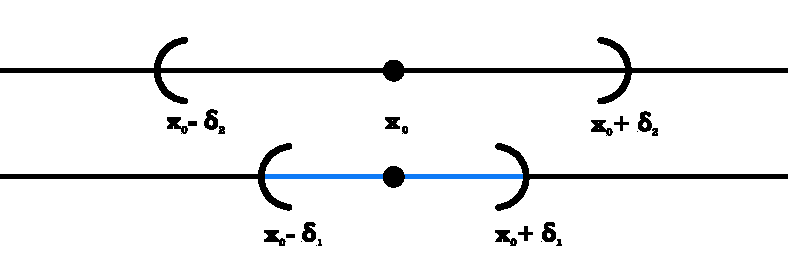
\includegraphics[width=12cm]{./images/interval2.pdf}
\end{figure}

\noindent\textbf{NB!} In generale, se interseco un numero \textbf{finito} di intorni di un certo numero reale $x_0$, ottengo ancora una volta un intorno di quel numero. Lo stesso avviene se interseco più intorni di $+\infty$ (o $-\infty$). Questo discorso però potrebbe non valere quando interseco infiniti intorni.\\

\noindent\textbf{ES.} Prendiamo $x_0 = 0$ e $A_n = D\left(0, \dfrac{1}{n}\right)$ con $n \in \mathbb{N}, n \geq 1$. Il nostro obiettivo è dimostrare che

\begin{equation*}
    B = \underset{\underset{\scriptstyle n \geq 1}{n \in \mathbb{N}}}{\cap} A_n = \{0\}
\end{equation*}

\noindent ovvero che l'intersezione dei vari intorni $A_n$ al variare di $n$ con $n \in \mathbb{N}, n \geq 1$ faccia esattamente $0$. Dividiamo la dimostrazione in due step: innanzitutto, proviamo che $A_n \supseteq \{0\}$ e successivamente che $A_n \subseteq \{0\}$ (in questo modo poi è possibile dire che $A_n = \{0\}$).\\
Partiamo dalla "$\supseteq$", ovvero mostriamo che $0 \in B$. Secondo la definizione di $B$ data precedentemente, ciò risulta equivalente a mostrare che $0$ appartiene a tutti gli insiemi $A_n$. In simboli: $0 \in A_n \quad \forall n \in \mathbb{N}, n \geq 1$. Dato che tutti gli $A_n$ sono centrati in $0$ (perché $A_n = D(0, \frac{1}{n})$), allora:

\begin{equation*}
     0 \in \underset{\underset{\scriptstyle n \geq 1}{n \in \mathbb{N}}}{\cap} A_n \implies \{0\} \subseteq \underset{\underset{\scriptstyle n \geq 1}{n \in \mathbb{N}}}{\cap} A_n
\end{equation*}

\noindent Procediamo ora con la seconda parte della dimostrazione ("$\subseteq$"). Sia $x > 0$ e per contraddizione diciamo che $x \in B$. Ciò significa però anche che $x \in A_n \quad \forall n \in \mathbb{N}, n \geq 1$. Ipotizziamo ora che:

\begin{equation}
    0 < x < \frac{1}{n} \qquad \forall n \in \mathbb{N}, n \geq 1
    \label{eq:11}
\end{equation}

\noindent Dato che l'insieme $\left\{\dfrac{1}{n} : n \geq 1\right\}$ è inferiormente limitato e, in particolare, $inf\left\{\dfrac{1}{n} : n \geq 1\right\} = 0$, ovvero $0$ è il massimo dei minoranti (abbiamo determinato tale valore utilizzando la proprietà di Archimede. Infatti $\forall \varepsilon > 0, \exists \Bar{n} \in \mathbb{N} \ | \ \Bar{n} > \frac{1}{\varepsilon} \implies \frac{1}{\Bar{n}} < \varepsilon$), in (\ref{eq:11}) se $x$ fosse minorante, allora $x \leq max(minoranti) \ (= 0)$, ovvero che $x \leq 0$. Arriviamo quindi ad una contraddizione. Ciò significa che nessun $x > 0$ può appartenere a $B$. \\
Allo stesso modo, sia $x < 0$ per contraddizione:

\begin{equation*}
    -\frac{1}{n} < x < 0 \qquad \forall n \in \mathbb{N}, n \geq 1
\end{equation*}

\noindent Definiamo ora $C = \left\{-\dfrac{1}{n} : n \in \mathbb{N}, n \geq 1\right\}$. Secondo questa definizione di $C$, $x$ rappresenta un maggiorante di questo insieme, ma per la proprietà di Archimede $sup(C) = 0$ (potevamo anche ricavarlo molto più semplicemente ricordandoci che $inf(-A) = -sup(A)$), dove $sup(C)$ è proprio il minimo dei maggioranti di $C$. Arriviamo però ancora una volta ad una contraddizione perché stiamo dicendo che esiste un maggiorante $x < 0$, che è più piccolo del minimo dei maggioranti ($0$). Per questo motivo, $x \geq 0$, quindi nessun $x < 0$ è appartenente a $B$.\\
Dato che come primo step abbiamo dimostrato l'appartenenza di $0$ a $B$ e dato che in questo secondo step abbiamo dimostrato che $B$ non contiene né $x < 0$, né $x > 0$, arriviamo alla conclusione che $B = \{0\}$. Riassumendo quindi presi infiniti intorni e intersecati tra di essi, otteniamo solo il loro centro (che ovviamente non è un intorno).

% PROVARE A FARE \CAP (N, + \INFTY) = \VARNOTHING...

\subsection{Teorema di unicità del limite}
Sia $f: A \subset \mathbb{R} \xrightarrow{} \mathbb{R}$ e $x_0 \in \widetilde{\mathbb{R}}$ con $x_0$ punto di accumulazione per $A$.\\
Suppongo che:

\begin{equation}
    \lim_{x\to x_0}f(x) = l_1 \in \widetilde{\mathbb{R}}
    \label{eq:12}
\end{equation}

\begin{equation}
    \lim_{x\to x_0}f(x) = l_2 \in \widetilde{\mathbb{R}}
    \label{eq:13}
\end{equation}

\noindent allora $l_1 = l_2$.

\subsubsection{Dimostrazione del teorema di unicità del limite}
Innanzitutto definiamo il primo limite (\ref{eq:12}). $\forall V_{l_1}$ intorno di $l_1$, $\exists U_{x_0}$ intorno di $x_0$ tale che $f(x) \in V_{l_1}$ per ogni $x \in (U_{x_0} \cap A) - \{x_0\}$.\\
Definiamo ora il secondo limite (\ref{eq:13}). $\forall V_{l_2}$ intorno di $l_2$, $\exists U'_{x_0}$ intorno di $x_0$ tale che $f(x) \in V_{l_2}$ per ogni $x \in (U'_{x_0} \cap A) - \{x_0\}$.\\

\noindent\textbf{NB!} Se $x_0 \in \{+\infty, -\infty\}$, non bisogna scrivere il $- \{x_0\}$ durante l'intersezione tra i due insiemi.\\

\noindent Supponiamo ora che $l_1 \neq l_2$. Allora $\exists V_{l_1}, V_{l_2}$ intorni di $l_1$ e $l_2$ rispettivamente tali che $V_{l_1} \cap V_{l_2} = \varnothing$.\\
Supponiamo ora che $l_1, l_2 \in \mathbb{R}$ e che $l_1 < l_2$. Possiamo quindi definire la distanza tra $l_2$ e $l_1$ come $d = l_2 - l_1 > 0$. Se prendiamo ora:

\begin{equation*}
    V_{l_1} = D\left(l_1, \frac{d}{2}\right) \qquad V_{l_2} = D\left(l_2, \frac{d}{2}\right)
\end{equation*}

\noindent abbiamo effettivamente che $V_{l_1} \cap V_{l_2} = \varnothing$. Graficamente:

\begin{figure}[!h]
    \centering
    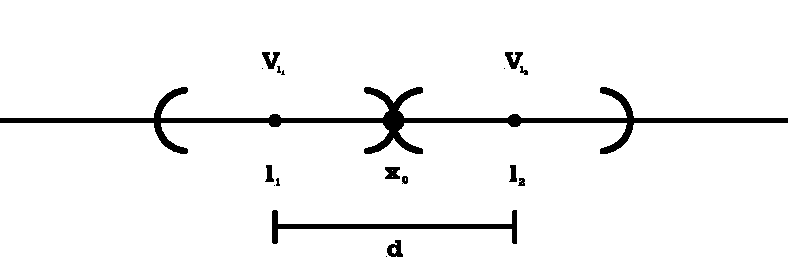
\includegraphics[width=12cm]{./images/interval3.pdf}
\end{figure}

% Mostrare per esercizio che funziona anche per l_1 = +\infty, l_2 \in \mathbb{R}; l_1 = -\infty, l_2 \in \mathbb{R}; l_1 = -\infty, l_2 = +\infty

\noindent Chiamiamo ora $W_{x_0} = U_{x_0} \cap U'_{x_0}$, che è un intorno di $x_0$. Sia $x \in (W_{x_0} \cap A) - \{x_0\} \neq \varnothing$ (perché $x_0$ è punto di accumulazione). Allora per la definizione di limite: $f(x) \in V_{l_1}$ (dato che $x \in W_{x_0} \subseteq U_{x_0}$ e se $x \in U_{x_0} \implies f(x) \in V_{l_1}$) e $f(x) \in V_{l_2}$ (dato che $x \in W_{x_0} \subseteq U'_{x_0}$ e se $x \in U'_{x_0} \implies f(x) \in V_{l_2}$). Quindi $f(x) \in V_{l_1} \cap V_{l_2}$, ma prima abbiamo preso apposta $V_{l_1}$ e $V_{l_2}$ tali che $V_{l_1} \cap V_{l_2} = \varnothing$. Siamo quindi arrivati ad una contraddizione. Ne deriva che $l_1 = l_2$ (nella pratica, infatti, non è possibile che una funzione sia arbitrariamente vicina sia ad un $l_1$ che ad un $l_2$ con $l_1 \neq l_2$. Allo stesso modo, se $l_1 = + \infty$ e $l_2 \in \mathbb{R}$, come fa $f(x)$ ad essere arbitrariamente vicina sia a $l_1$, che a $l_2$?!).

\end{document}